\documentclass[12pt,twoside]{thesis}

\usepackage{amssymb}
\usepackage{float}
\usepackage{subcaption}
\usepackage{varwidth}
\usepackage{environ}

\usepackage[framemethod=default]{mdframed}
\usepackage[linesnumbered,ruled,vlined]{algorithm2e}

\renewcommand{\baselinestretch}{1}
\setlength{\parskip}{0.25\baselineskip}

\NewEnviron{annexample}[5][]{
	\begin{figure}[H]
		\centering
		\begin{minipage}{\dimexpr #2\relax}
			\begin{mdframed}[linecolor=black,backgroundcolor=white,linewidth=1pt,#1]
				\texttt{\BODY}
			\end{mdframed}
		\end{minipage}
		\caption[#4]{#5}
		\label{#3}
	\end{figure}
}

% quotation
\newcommand{\doublequote}[1]{``#1''}
\newcommand{\guillemot}[1]{\guillemotleft#1\guillemotright}

% math abs
\newcommand{\abs}[1]{\left|#1\right|}

\title{Generación Automática de Ontologías}
\author{José Ariel Romero Costa}
\advisor{MSc. Juan Pablo Consuegra Ayala}
\degree{Licenciado en Ciencia de la Computación}
\university{Universidad de La Habana}
\faculty{Facultad de Matemática y Computación}
\date{Septiembre de 2020}
\logo{graphics/university_logo}
%\makenomenclature

\begin{document}
	\let\cleardoublepage\clearpage

	\frontmatter
	\maketitle

	% phrase
	\begin{flushright}
	\itshape
	\parbox[l]{2.9in}{
		-- Sólo se vive una vez, y ya hice mi elección.\\
		-- ¡Error!, sólo se muere una vez; vivimos\\todos los días. Además, no importa cuánto tiempo hayas viajado en la dirección equivocada, siempre puedes cambiar de dirección.
	}
\end{flushright}

	% dedication
	%===================================================================================
% Chapter: Phrase
%===================================================================================

\begin{phrase}[4.2in]
	Dedicado a mis padres, Ramón y Amparo, quienes han batallado a mi lado incansablemente y de forma incondicional durante estos $23$ años de vida y $18$ años de estudio.\\
	A Julio, mi hermano, quien siempre ha estado certero con sus consejos y apoyándome en todo lo que he necesitado fuera y dentro del ámbito educacional.\\
	A Odalmis, mi novia, prometida y próximamente esposa, hemos cursado los buenos y malos momentos en en estos últimos $4$ años y ha estado siempre presente para dar un consejo o apoyo cuando lo necesito.\\
	A todo aquel que, sin importar si fue un simple \doublequote{buenos días}, una charla pasajera o esporádica o una larga amistad de años, intervino en mi vida para hacer de mí lo que soy hoy.
\end{phrase}

	% thanks
	thanks

	% supervisor opinion
	%===================================================================================
% Chapter: Supervisor Opinion
%===================================================================================

\begin{opinion}
	La representación de conocimiento se ha convertido en un área de investigación muy activa en los últimos años, motivada tanto por la disponibilidad masiva de nuevos recursos, como por la necesidad de hacer computacionalmente tratable el volumen de datos producidos diariamente. Su relevancia en tareas más amplias, como el descubrimiento automático de conocimiento, la vuelven un área crucial para el desarrollo de varios sectores de la sociedad. En el dominio médico, la aplicación de estas técnicas se vuelve especialmente interesante, ya que procedimientos de inferencia sobre una base de conocimiento puede potencialmente ayudar a diseñar nuevos tratamientos para combatir enfermedades aún no resueltas. En este marco se desarrolla la tesis de licenciatura de José Ariel Romero Costa, con quien pude trabajar este último año en el diseño y validación de un algoritmo para la construcción de ontologías a partir de textos anotados. Esta tesis da continuidad a una línea de investigación que se ha venido desarrollando en la facultad en los últimos años ligada al descubrimiento de conocimiento.

	La propuesta de José consiste en un algoritmo para la creación automática de ontologías a partir de una colección anotada de documentos. El sistema utiliza el esquema de anotación del \emph{eHealth-KD Challenge} que ha sido empleado en dos competencias internacionales de extracción de conocimiento, en el marco de los eventos \emph{IberLEF 2019} e \emph{IberLEF 2020}. El trabajo conllevó reconstruir un corpus de texto de Medline sobre el que identificar y reordenar las oraciones del corpus anotado. A partir de las entidades y relaciones señaladas en el texto, se realiza un proceso de normalización con el objetivo de unificar aquellas entidades que difieren sintácticamente pero comparten la misma semántica. La tesis presenta un procedimiento para organizar la información recogida en múltiples oraciones, formando una base de conocimiento que integra las distintas instancias de anotaciones mencionadas entre colecciones. La representación final obtenida constituye un paso de avance en la formalización del esquema de anotación, y sienta las bases para futuros procesos de inferencia.

	Durante el desarrollo de la tesis José demostró independencia y creatividad para lidiar con los problemas encontrados. Tuvo que dominar conceptos y tecnologías del estado del arte, con muchas de las cuales no tuvo contacto durante la carrera. Los problemas que hubo de resolver le servirán de aprendizaje para su desarrollo futuro. El proceso de investigación e implementación desarrollado por José queda recogido en un documento de tesis que avala la capacidad adquirida para presentar resultados de investigación de forma concisa y coherente. Todo esto lo han realizado a la par de las actividades docentes, como estudiante de pregrado y como alumno ayudante de la asignatura \emph{Programación}, donde ha sabido asumir con éxito todas las responsabilidades y retos.

	José ha sido alumno ayudante desde su tercer año en la carrera, tiempo que pude compartir con él directamente en clases y en las reuniones del colectivo. En esos años he podido comprobar su interés y dedicación por la asignatura y otros temas relacionados. Este último ejercicio demuestra que ya ha adquirido la madurez necesaria para desarrollar proyectos de alta complejidad con calidad y esmero. Como tutor, estoy complacido por los resultados obtenidos, y por el trabajo realizado con José, que aunque no estuvo exento de obstáculos, logró superar los desafíos. Por estos motivos estoy convencido de que José será un excelente profesional de la Ciencia de la Computación.

	\vspace{1cm}
	\begin{flushright}
		\emph{MSc. Juan Pablo Consuegra Ayala}\\
		Facultad de Matemática y Computación\\
		Universidad de La Habana
	\end{flushright}
\end{opinion}

	% abstract (spanish)
	%===================================================================================
% Chapter: Abstract (spanish)
%===================================================================================
\ChapterOutOfToc{Resumen}\label{chapter:abstract_spanish}
%===================================================================================

En los últimos años se ha evidenciado un aumento en el desarrollo de técnicas para descubrir conocimiento de forma automática en documentos escritos en lenguaje natural. El procesamiento automático va aparejado a la posibilidad de analizar colecciones de información con disímiles textos. En el área de la medicina, el auge de estas tecnologías es especialmente significativo, pues permite favorecerse de la gran cantidad de información disponible para el avance de este campo, que posee gran importancia para la sociedad. Por otra parte, estas técnicas suelen apoyarse en corpus anotados, los cuales son recursos escasos. Esto se vuelve crítico en el idioma español, donde la cantidad existente es ínfima y de dominio menos generalizado.

En este estudio se define un modelo de anotación de propósito general con el objetivo de capturar los rasgos semánticos más relevantes en los documentos de texto. Además, se presenta un esquema de ontología que se usará para la extracción de conocimiento de forma automática. También se ofrecen los pasos a seguir para la implementación de un algoritmo computacional que busca representar un corpus anotado como un grafo de conocimiento, siguiendo las reglas definidas por la propia ontología. Por último, se muestran las tareas realizadas para la validación de las propuestas dadas, así como resultados en términos matemáticos.

Los resultados alcanzados demuestran que el descubrimiento de conocimiento constituye un campo de investigación activo, donde pueden aplicarse técnicas de aprendizaje automático logrando resultados positivos. Se propone la verificación y comparación de un grafo de conocimiento específico creado a partir de las propuestas brindadas en este estudio respecto a la capacidad de aprendizaje e interpretación de un grupo de expertos en el mismo tema. Además se ofrece la continuación de esta línea de investigación con el objetivo de mejorar la efectividad de las propuestas dadas y su aplicación en otros dominios.

	% abstract (english)
	%===================================================================================
% Chapter: Abstract (english)
%===================================================================================
\ChapterOutOfToc{Abstract}\label{chapter:abstract_english}
%===================================================================================

\hyphenation{de-fined}
\hyphenation{ex-posed}
\hyphenation{knowl-edge}
\hyphenation{scheme}

In recent years there has been an increase in the development of techniques for automatic knowledge discovery from documents written on natural language. Automatic processing provides the possibility to analyze collections of information containing a large number of texts. In the medical field, the rise of these technologies is significantly special, because it allows taking advantage of the huge amount of data available for it and improve research on this area, which is really important to society. These techniques tend to rely on annotated corpus, and they are a scarce resource. This becomes a critical fact in Spanish language, where the existing amount of them is very low and from a less general domain.

In this study, a general-purpose annotation model is defined to capture the most relevant semantic features contained in text documents. Also, an ontology scheme is presented and used for automatic knowledge extraction. A theoretical step by step implementation of a computational algorithm aiming to build a knowledge graph from an annotated corpus and following the rules of the previously defined ontology is also proposed. Finally, the evaluation and validation process is exposed, as well as statistics results.

The results achieved demonstrate that knowledge discovery constitutes an active research field, where machine learning techniques can be applied achieving positive results. The verification and comparison of a specific knowledge graph built from the proposals provided in this investigation against the learning and interpretation skills of a group of experts on the same field is proposed. Also, the continuation of this research line is suggested, aiming to improve the effectiveness of the proposals given and their application in other domains.

	% contents
	%===================================================================================
% Chapter: Contents
%===================================================================================

\tableofcontents
\listoffigures
\listoftables

	\mainmatter

	% introduction
	%===================================================================================
% Chapter: Introduction
%===================================================================================
\Chapter*{Introducción}\label{chapter:introduction}
%===================================================================================

\hyphenation{herra-mien-tas}
\hyphenation{corre-la-cio-nar-los}

El desarrollo tecnológico se ha exacerbado con el advenimiento cada vez mayor del uso del Internet y otros medios avanzados y efectivos que garantizan un mejor futuro para cuestiones importantes de la vida. Debido al continuo aumento del flujo informativo, se hace cada vez más necesaria la utilización de herramientas que permitan identificar, capturar y representar el conocimiento dentro de los sistemas de información, ya sea de dominio específico o de propósito general.

Para ello, ciencias avanzadas como la Ciencia de la Computación y de la Comunicación comprenden la ontología como la definición de conceptos y relaciones en algún dominio, de forma compartida y consensuada. Esta conceptualización debe ser representada de una manera formal, legible y utilizable por los ordenadores~\cite{ref:30}. Son creadas para limitar la complejidad de cualquier tema y para organizar la información. Es una medida eficaz en las soluciones de problemas comunes en la vida diaria, que debido a la sobreinformación no se podrían llevar a cabo de forma manual.

Otro de sus beneficios es el hecho de que permiten crear entendimiento compartido al unificar los diferentes puntos de vista. Esto sirve para facilitar la comunicación entre los actores implicados en la construcción de sistemas de información referidos al dominio. Además, permiten el reuso del conocimiento del tema, pues sirve de base ya creada para posteriores investigaciones. También facilitan la recuperación, integración e interoperatividad entre fuentes de conocimiento heterogéneas. Con ellas se provee una base para la representación del conocimiento del dominio y ayudan a identificar las categorías semánticas del mismo~\cite{ref:1}.

Surge entonces el creciente interés de estudiar técnicas para el descubrimiento automático de conocimiento. El procesamiento automático trae consigo la posibilidad de analizar colecciones masivas de información. Sin embargo, la mayor parte de estas colecciones almacenan la información disponible en documentos textuales escritos en lenguaje natural. La naturaleza en que se expresa la información y su estructura semántica poco unificada se vuelven la principal fuente de retos de dicho procesamiento.

En la actualidad, las ontologías se están aplicando en áreas heterogéneas. Entre ellas se encuentran la búsqueda de información, el comercio electrónico, configuraciones de aplicaciones o productos. Además, todo sitio web grande debería usarlas, al menos para organización y navegación~\cite{ref:31}. También se están utilizando para el desarrollo de mecanismos que faciliten la comunicación entre las personas y las máquinas por medio del lenguaje natural~\cite{ref:2}.

En el contexto de la salud y la medicina las ontologías adquieren particular interés, debido a que se están utilizando cada vez más para la solución de disímiles tareas, como la recuperación de información y la búsqueda de respuestas en fragmentos de texto que resuelven preguntas. Diariamente se publican muchos artículos médicos y se hace imposible acceder a todos y obtener conocimiento sobre las novedades médicas y las herramientas que se van desarrollando para solucionar las enfermedades o los problemas de la salud de manera general.

La extracción automática de conocimiento proveería de una herramienta para asistir el desarrollo en esta área a partir de la normalización e integración de los resultados encontrados. Una vez extraído y representado el conocimiento computacionalmente, procesos de inferencia permitirían el descubrimiento de nuevo conocimiento. Ejemplo de esto es el constante descubrimiento de nuevas interacciones entre medicamentos, proteínas y genes. Un sistema de descubrimiento de conocimiento posibilitaría la detección automática de
nuevas relaciones entre ellos, y por ende, el descubrimiento de nuevas causas de enfermedades, síntomas y tratamientos.\\

Algunas de las razones principales para el desarrollo de una ontología son:

\begin{itemize}
	\item[•] Compartir conocimiento de la estructura de la información entre investigadores y/o usuarios.
	\item[•] Permitir la reutilización del conocimiento del dominio.
	\item[•] Hacer explícitas las suposiciones o conocimientos a priori del dominio.
	\item[•] Separar el conocimiento explícito del dominio del conocimiento implícito operacional.
	\item[•] Analizar el conocimiento del dominio.
\end{itemize}

\textit{Compartir conocimiento de la estructura de la información entre investigadores y/o usuarios} es uno de los objetivos comunes en el desarrollo de ontologías~\cite{ref:4,ref:10}. Por ejemplo, si varios sitios web diferentes entre sí contienen información médica o proporcionan servicios médicos de comercio electrónico, y estos comparten y publican la misma ontología subyacente de los términos que utilizan, los agentes informáticos pueden extraer y agregar información de los mismos. Además, estos últimos pudieran utilizar dicha información para responder consultas de los usuarios o como datos de entrada para otras aplicaciones.

\textit{Permitir la reutilización del conocimiento del dominio} fue una de las fuerzas impulsoras detrás del reciente aumento de la investigación ontológica. Por ejemplo, los modelos para muchas áreas diferentes deben representar la idea de tiempo. Esta representación incluye, entre otros, las nociones de intervalos, puntos y medidas relativas a este. Si un grupo de investigadores desarrolla tal ontología en detalle, otros pueden simplemente reutilizarla para sus dominios. Además, si se necesita construir una grande, se pueden integrar varias ya existentes que describan partes específicas de la rama deseada. También se puede reutilizar una de propósito general, como UNSPSC, y extenderla para describir el área de interés.

\textit{Hacer explícitas las suposiciones o conocimientos a priori del dominio} hace posible cambiarlas fácilmente si cambian las ideas tenidas de antemano en este tema. Los supuestos de \textit{codificación rígida} (del inglés \textit{hard-coding}) sobre el mundo hechos en lenguajes de programación hacen que estas no solo sean difíciles de encontrar y comprender, sino también de cambiar, en particular para alguien sin experiencia en el ámbito computacional. Además, las especificaciones explícitas del conocimiento del dominio son útiles para los nuevos usuarios que deben aprender qué significan los términos de este.

\textit{Separar el conocimiento explícito del dominio del conocimiento implícito operacional} es otro uso común de las ontologías. Se puede describir la tarea de configurar un producto a partir de sus componentes, de acuerdo con una especificación requerida e implementar un programa que realice esta configuración independientemente del producto~\cite{ref:11}. Seguido de esto, se puede desarrollar una ontología de componentes y características de los ordenadores personales y aplicar el algoritmo para configurar uno de ellos a medida~\cite{ref:12}.

\textit{Analizar el conocimiento del dominio} es posible una vez se disponga de una especificación declarativa de los términos. El análisis formal de estos es extremadamente valioso cuando se intenta reutilizar ontologías existentes y ampliarlas~\cite{ref:13}.

\noindent\textbf{\large Problemática}

En disímiles ocaciones, es necesaria la lectura de un amplio grupo de documentos con gran cantidad de páginas para poder tener conocimiento acerca de algún tema. Incluso algunas veces la información leída no es relevante para lo que se desea, y por tanto, fue una inversión de tiempo en vano. Las ontologías, por otra parte, aceleran en gran medida este proceso, pues el análisis y representación de uno o más corpus en un grafo de conocimiento es cuestión de segundos. Esto posibilita posteriormente, buscar la información deseada a través de consultas realizadas a un sistema computacional.

Para diseñar una ontología no existe una única forma o metodología correcta a emplear y tampoco es objetivo de este estudio definir una. Con esta investigación se busca dar solución al problema de representar un corpus de documentos anotados como base de conocimiento, por medio de una ontología. Para ello es necesaria la definición de la propia ontología a usar y un algoritmo computacional que posibilite la realización de este proceso.

La generación de ontologías es un proceso que de ser realizado de forma manual, toma demasiado tiempo y esfuerzo. Además, en aras de completar la construcción de una base de conocimientos medianamente buena o buena, es necesario involucrar expertos en el dominio. Por otra parte, estas restricciones imposibilitan la realización de una ontología para todos los posibles corpus de estudio. En cambio, con esta investigación se busca realizar este proceso de forma totalmente automática, sin la necesidad tener conocimiento previo del dominio y tras la espera de unos pocos segundos puede verse el resultado de la ontología construida.

Este problema lleva implícito el procesamiento de lenguaje natural, pues en este están escritos los corpus de documentos que serán usados. Además, el campo de estudio de la generación automática de ontologías es relativamente moderno. Este conjunto de aspectos lo hace ser un problema interesante. Es por esto que es el objetivo de esta investigación.

En esta investigación, además de definir un esquema de ontología de propósito general, se lleva a cabo la realización de una base de conocimiento mediante la utilización de un corpus de dominio médico extraído de \textit{Medline}~\cite{ref:3}.\\

\noindent\textbf{\large Objetivos}

La investigación se plantea como objetivo general definir un diseño de ontología de propósito general que sea capaz de representar el conocimiento descrito en uno o más corpus anotados.

Para darle solución al objetivo general es necesaria la implementación de un algoritmo computacional capaz de representar uno o más corpus de documentos anotados como un grafo de conocimiento que responde a las reglas establecidas por la ontología propuesta.

Se proponen los siguientes objetivos específicos:
\begin{itemize}
	\vspace{-0.27cm}
	\item[•] Estudiar los esquemas de anotación y corpus usados en diversas tareas de extracción del conocimiento.
	\vspace{-0.27cm}
	\item[•] Definir un esquema conceptual de anotación para la representación de los rasgos semánticos más relevantes en textos escritos en lenguaje natural.
	\vspace{-0.27cm}
	\item[•] Definir un formato de anotación de archivos para el esquema conceptual previamente definido.
	\vspace{-0.27cm}
	\item[•] Diseñar una propuesta de ontología donde se pueda representar un corpus de documentos escritos en lenguaje natural.
	\vspace{-0.27cm}
	\item[•] Implementar un algoritmo computacional para representar un corpus anotado como grafo de conocimiento a través de dicha ontología.
	\vspace{-0.27cm}
	\item[•] Implementar un marco experimental para la evaluación de la propuesta de solución.
\end{itemize}

\noindent\textbf{\large Organización de la tesis}

El contenido de la tesis se organiza de la siguiente forma. El capítulo \ref{chapter:automatic_generation_of_ontologies} introduce los principales conceptos relacionados con las ontologías y la extracción y representación de conocimiento. En este capítulo, además, se analizan los principales corpus y representaciones semánticas existentes en la literatura. El capítulo \ref{chapter:annotation_model} describe un modelo de anotación de propósito general que busca capturar los rasgos semánticos más importantes en documentos de texto. En el capítulo \ref{chapter:proposed_solution} se presenta una propuesta para la creación de un grafo de conocimiento a través de un corpus anotado. En el capítulo \ref{chapter:analysis_of_results} se muestran los resultados alcanzados en esta investigación, y en función de estos, se discute la efectividad de cada uno de los elementos propuestos en la misma. La investigación finaliza presentando las conclusiones pertinentes y las recomendaciones para su continuidad y mejora.

	% ontology learning
	%===================================================================================
% Chapter: Ontology Learning
%===================================================================================
\chapter{Aprendizaje de Ontologías}\label{chapter:ontology-learning}
%===================================================================================


	% annotation model
	%===================================================================================
% Chapter: Annotation model
%===================================================================================
\chapter{Modelo de anotación}\label{chapter:corpus-description}
El primer paso para el algoritmo presentado en este trabajo, es tener un corpus\footnote{Un corpus es un conjunto de oraciones y/o documentos de ejemplos reales usados en el lenguaje natural.} anotado basado en el esquema presentado a continuación. Además, en este capítulo son analizadas varias estadísticas de un corpus de oraciones del dominio médico en idioma español, el cual es utilizado en la presente investigación y son mostradas las herramientas empleadas para construirlo y trabajar con el mismo.

%===================================================================================

\section{Esquema de Anotación}
El modelo de anotación de propósito general empleado busca capturar los rasgos y relaciones semánticas más relevantes presentes en oraciones del lenguaje natural. Este debe evitar ambigüedades tanto como sea posible, de forma que anotadores humanos distintos tengan una alta probabilidad de coincidir. Necesita ser lo suficientemente expresivo para capturar los conceptos relevantes del dominio y sus interacciones. Además, debe ser capaz de representar conceptos complejos a partir de combinar otros más simples, esto permitiría construir conceptos mucho más complejos que los que se nombran directamente en el texto con un conjunto reducido de reglas. También está diseñado para asistir en la construcción de sistemas de descubrimiento de conocimiento. Por este motivo es necesario independizar la representación del modelo de la estructura gramatical de las oraciones, y en su lugar tratar de representar su significado semántico.

Este modelo de anotación se basa en las tripletas \textit{Subject-Action-Target} (en español \textit{Sujeto-Acción-Objetivo}) y además en la estructura gramatical \textit{sujeto-verbo-objeto}, normalmente expresada con su abreviatura \textbf{SVO} y es el orden más usado en los idiomas del mundo. Tiende a ser el orden predeterminado porque el verbo se usa para dividir el sujeto del predicado, sin necesidad de usar partículas para indicar dónde empieza o terminan los mismos. Es, por ende, una de las secuencias más frecuente en el lenguaje natural y de hecho es usada en la mayoría de lenguas occidentales y un buen número de orientales.

\begin{figure}[h!]
	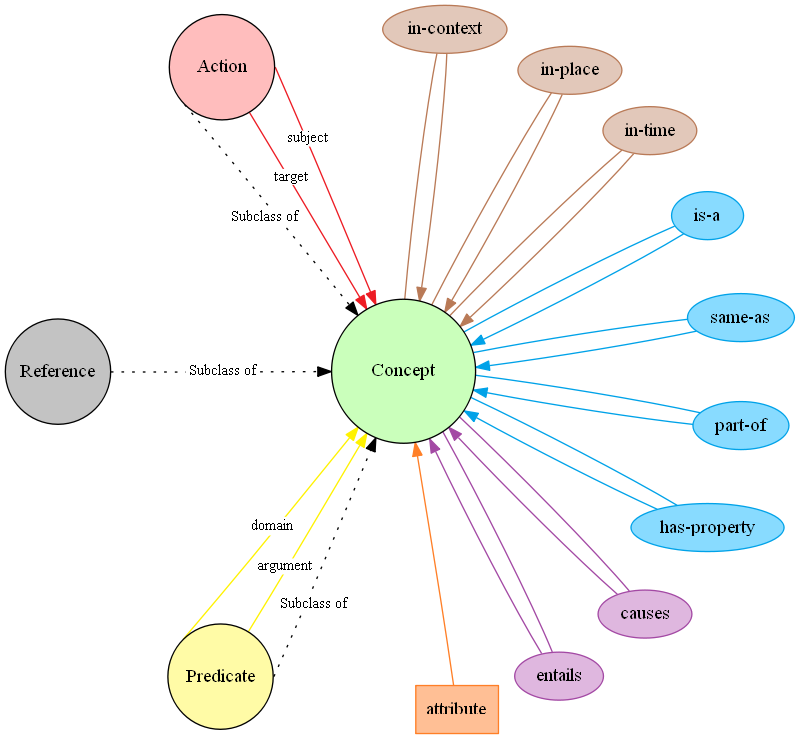
\includegraphics[width=\linewidth]{graphics/annotation_model.png}
	\caption[Esquema conceptual del modelo de anotación]{Esquema conceptual del modelo de anotación.}
	\label{fig:annotation_model}
\end{figure}

Es válido destacar que al estar interesados en fragmentos de conocimiento, el rol semántico de las entidades anotadas puede no coincidir con su rol gramatical. Los roles semánticos fundamentales de este modelo son \textit{Concept} y \textit{Action} (en español \textit{Concepto} y \textit{Acción} respectivamente), siendo usados para representar información objetiva acerca de lo que está siendo hecho, por quién, y a quién. Estas estructuras pueden ser contextualizadas en tiempo, lugar y otras circunstancias generales.

Existen otros 2 roles semánticos, llamados \textit{Predicate} y \textit{Reference} (en español \textit{Referencia} y \textit{Predicado} respectivamente). \textit{Predicate} es utilizado para construir conceptos más complejos a partir de otros más simples. \textit{Reference} define un término del que se menciona un hecho, pero en el contexto de la oración no está escrito explícitamente, por lo que la información semántica de estas anotaciones no está contenida en las anotaciones.

Por último, son usadas seis relaciones con semántica específica para representar conocimiento de propósito general. Las relaciones
\textit{is-a}, \textit{part-of}, \textit{same-as} y \textit{has-property} (en español \textit{es-un}, \textit{parte-de}, \textit{igual-que} y \textit{tiene-propiedad} respectivamente) son tomadas de representaciones ontológicas y taxonómicas, mientras que \textit{causes} y \textit{entails} (en español \textit{causa} e \textit{implica} respectivamente) se toman del dominio de la comprensión del texto. Además, las relaciones \textit{in-time}, \textit{in-place} e \textit{in-context} (en español \textit{en-tiempo}, \textit{en-lugar} y \textit{en-contexto} respectivamente) son usadas para dar contexto y cuatro atributos booleanos son asociados a los conceptos. Las próximas secciones explican cada rol semántico y las relaciones detalladamente, incluyendo ejemplos de su uso en oraciones del lenguaje natural.

La figura \ref{fig:annotation_model} muestra una representación gráfica del modelo de anotación. En el esquema conceptual se puede apreciar que cada uno de los roles semánticos definidos en el modelo de anotación está representado por un círculo. Además, las posibles relaciones definidas entre cada pareja de roles se representan con óvalos y con un rectángulo los atributos que pueden tener los roles semánticos. En color café están representadas las relaciones de contexto, en azul las taxonómicas y en violeta las de causalidad e implicación.

\subsection{Conceptos}
El rol \textit{Concept} es usado para anotar fragmentos de texto que representan una unidad atómica de información en el dominio. Puede ser una entidad nombrada, un sustantivo, adjetivo o verbo, que representa un concepto relevante en el dominio del texto. Por ende, la gran mayoría de palabras o frases que expresan un significado propio es anotado como \textit{Concept} (o uno de sus derivados, como se explica más adelante). Palabras tales como artículos, preposiciones y conjunciones, las cuales solo realizan una función gramatical y sin significado semántico, no son anotados.

\begin{figure}[h]
	\begin{center}
		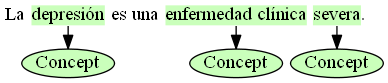
\includegraphics[width=3.5in]{graphics/annotation_example_concept.png}
		\caption[Anotación de conceptos]{Ejemplo de anotación de conceptos.}
		\label{fig:annotation_example_concept}
	\end{center}
\end{figure}

En la figura \ref{fig:annotation_example_concept} se distinguen claramente las palabras \guillemot{\texttt{depresión}} y \guillemot{\texttt{severa}} como conceptos en el dominio médico, cuyo significado de cada uno de ellos es independiente del rol gramatical que tengan en la oración. Algunos conceptos, como \guillemot{\texttt{enfermedad clínica}} en este caso, se componen de múltiples palabras, ya sea porque las palabras individuales que lo componen no tengan significado por sí mismas, o porque el concepto formado por su unión es diferente de sus significados individuales. En esta ocasión, a pesar de que \guillemot{\texttt{enfermedad}} y \guillemot{\texttt{clínica}} poseen un significado individual bien definido, el concepto \guillemot{\texttt{enfermedad clínica}} tiene su significado bien definido en el dominio médico, lo cual lo hace una unidad única de información, en otras palabras, un especialista del dominio puede identificarla claramente. Las palabras que conforman el concepto no tienen que estar consecutivas en el texto, pero sí son seleccionadas de izquierda a derecha.

\subsection{Acciones}
El rol \textit{Action} es un tipo particular de \textit{Concept} que indica una acción o evento que otro concepto puede realizar o ser objetivo de ella. Un \textit{Action} puede ser enlazado con otros conceptos relevantes a partir de 2 roles semánticos: \textit{subject} y \textit{target} (en español \textit{sujeto} y \textit{objetivo} respectivamente). El \textit{subject} es el concepto que produce la acción, mientras que el \textit{target} es el concepto que recibe los efectos o es el objetivo de la acción.

\begin{figure}[H]
	\begin{center}
		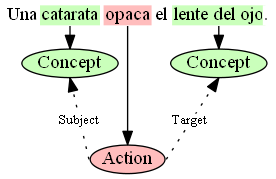
\includegraphics[height=1.7in]{graphics/annotation_example_action.png}
		\caption[Anotación de acción]{Ejemplo de anotación de acción.}
		\label{fig:annotation_example_action}
	\end{center}
\end{figure}

En la figura \ref{fig:annotation_example_action} la acción es indicada por una palabra con el rol gramatical de verbo. Intuitivamente este es el caso más común, sin embargo, una acción puede ser indicada además por una palabra con otro rol gramatical, como los sustantivos. Por ejemplo, en la frase \doublequote{\textit{\dots\space el empeoramiento de los síntomas \dots}}, la palabra \guillemot{\texttt{empeoramiento}} se considera también un \textit{Action} a pesar de que no es un verbo, dado que describe un proceso o evento que ocurre sobre otros conceptos.

Por tanto, el rol semántico \textit{Action} describe el significado de un concepto en el dominio semántico, en lugar de su función gramatical en una oración específica. Si un concepto del dominio expresa un proceso o evento que realiza un concepto o produce un efecto sobre otro(s), entonces es un \textit{Action}, incluso si puede ser usado con una función gramatical distinta.

\subsection{Referencias}
El rol \textit{Reference} es un tipo de \textit{Concept} que no tiene un significado semántico específico, pero que es necesario por razones gramaticales. Es usado para anotar pronombres (por ejemplo, \textit{este}, \textit{aquel}) y demás elementos que hacen referencia a otro \textit{Concept} presente en la oración, documento y/o corpus. En la figura \ref{fig:annotation_example_reference_and_predicate} puede verse un ejemplo.

\subsection{Predicados}
El rol \textit{Predicate} es usado para formar conceptos más complejos a partir de aplicar un determinado criterio sobre otros conceptos en una oración. Un caso de uso común es para definir el subconjunto de un concepto que cumple determinadas propiedades.

\begin{figure}[H]
	\begin{center}
		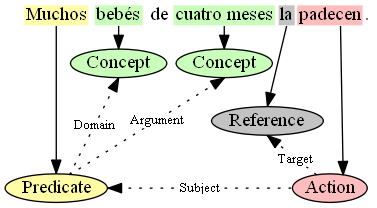
\includegraphics[width=3.4in]{graphics/annotation_example_reference_and_predicate.png}
		\caption[Anotación de referencia y predicado]{Ejemplo de anotación de referencia y predicado.}
		\label{fig:annotation_example_reference_and_predicate}
	\end{center}
\end{figure}

\vspace{-0.04in}
Por ejemplo, en la figura \ref{fig:annotation_example_reference_and_predicate}, la palabra \textit{muchos} cumple la función de filtrar algunos de los bebés, por eso es anotada como \textit{Predicate}.

De conjunto con esta relación, cualquier concepto puede jugar dos roles adicionales: \textit{domain} y \textit{argument} (en español \textit{dominio} y \textit{argumento} respectivamente), completando así su significado. El \textit{Predicate} define el conjunto de objetos pertenecientes al dominio (el concepto enlazado con el rol \textit{domain}) que cumplen el predicado anotado según los argumentos señalados (el o los conceptos anotados con el rol \textit{argument}). De forma matemática, la relación \textit{Predicate} define al conjunto:

\begin{center}
	$\{x\in Domain~|~Predicate(x,~arg_1,~arg_2,\dots,~arg_n)\}$
\end{center}

En el ejemplo de la figura \ref{fig:annotation_example_reference_and_predicate}, el dominio de este \textit{Predicate} es representado por el \textit{Concept} \guillemot{\texttt{bebés}}, y el único argumento es \guillemot{\texttt{cuatro meses}}. Esta construcción da lugar a un nuevo concepto, el de muchos bebés de 4 meses, el cual puede ser entendido como la aplicación del filtro \guillemot{\texttt{muchos}} sobre el conjunto de elementos
definido por el \textit{Concept} \guillemot{\texttt{bebés}}, de los cuales son seleccionados aquellos con el argumento \guillemot{\texttt{cuatro meses}}.

\begin{center}
	$\{x\in Beb\acute{e}s~|~muchos(x,~cuatro~meses)\}$
\end{center}

El nuevo concepto complejo construido de esta forma es representado
en la oración por la anotación \textit{Predicate} en sí misma. Por tanto, para continuar con el ejemplo anterior, en caso de querer que estos \guillemot{\texttt{muchos bebés}} jugaran el rol \textit{subject} o \textit{target}, la anotación correspondiente debe ir desde un \textit{Action} hacia el \textit{Predicate}, como se muestra en la figura \ref{fig:annotation_example_reference_and_predicate}. Es un error anotar que el \textit{subject} de \guillemot{\texttt{padecen}} es \guillemot{\texttt{bebés}} porque este concepto representa \doublequote{todos los bebés}. Por ende, el \textit{Predicate} es usado para representar el concepto filtrado en sí, no el operador de filtrado.

Como caso de uso particular de esta anotación, se encuentra el caso en que un término no representa un concepto relevante por sí mismo (por tanto no debe ser anotado como \textit{Concept}), sino que denota una propiedad o rasgo medible de otro concepto. Por ejemplo, \guillemot{\texttt{tipo}}, \guillemot{\texttt{parte}}, \guillemot{\texttt{nivel}} y \guillemot{\texttt{cada}} en \doublequote{\textit{tipo de cáncer}}, \doublequote{\textit{parte del cuerpo}}, \doublequote{\textit{nivel de glucosa}} y \doublequote{\textit{cada trimestre}} respectivamente.
En tales casos, el \textit{Predicate} debe carecer de alguno de los roles \textit{domain} o \textit{argument}. Si el tipo o clase resultante de formar el predicado coincide con el del concepto a enlazar, entonces el rol utilizado es \textit{domain}. En otro caso, se enlaza al concepto con el rol \textit{argument}.

\subsection{Componiendo conceptos}
Así como un \textit{Predicate} puede utilizarse para componer conceptos, se puede lograr un resultado similar al considerar un \textit{Action} como el \textit{subject} o \textit{target} de otro.

\begin{figure}[H]
	\begin{center}
		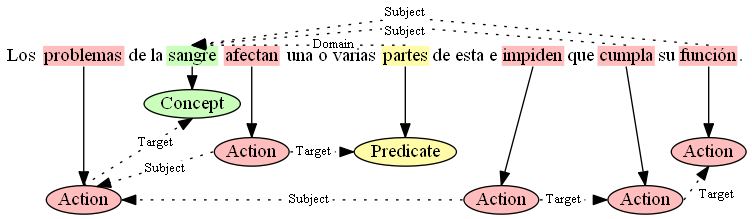
\includegraphics[width=\linewidth]{graphics/annotation_example_composing_concepts.png}
		\caption[Anotación de conceptos compuestos]{Ejemplo de anotación de conceptos compuestos.}
		\label{fig:annotation_example_composing_concepts}
	\end{center}
\end{figure}

Por ejemplo, en la figura \ref{fig:annotation_example_composing_concepts}, hay un concepto complejo
que involucra a \guillemot{\texttt{problemas}} y \guillemot{\texttt{sangre}}. Este concepto actúa como \textit{subject} de \guillemot{\texttt{afectan}}, dado que no todos los \guillemot{\texttt{problemas}} se \guillemot{\texttt{afectan}}, sino solo aquellos que son \guillemot{\texttt{problemas de la sangre}}. Por otro lado, la propia palabra \guillemot{\texttt{sangre}} actúa como \textit{domain} del predicado \guillemot{\texttt{partes}}. Quien a su vez es el \textit{target} de \guillemot{\texttt{afectan}}. De manera similar sucede con los otros tres conceptos complejos \guillemot{\texttt{impiden}}, \guillemot{{cumpla}} y \guillemot{\texttt{función}}.

De esta forma puede apreciarse que la construcción y/o anotación de conceptos complejos es una tarea compleja en sí. Además, esta estrategia puede ser usada para representar la nominalización de un verbo, pues al anotar el \textit{Action} y los correspondientes \textit{subject} y \textit{target} se
construye el concepto complejo.

\subsection{Relaciones taxonómicas}
Los roles \textit{Action} y \textit{Concept} permiten capturar gran parte del significado semántico de una oración a partir de anotar como acción todos los conceptos que indican alguna interacción entre otros conceptos. Sin embargo, algunos tipos específicos de interacciones son tan comunes que son considerados en diferentes dominios del conocimiento como los bloques constructores para las representaciones ontológicas y taxonómicas. Tal es el caso de las parejas de hiperonimia/hiponimia, anotadas como relaciones \textit{is-a} (en español \textit{es-un}) y meronimia/holonimia, anotadas como relaciones \textit{part-of} (en español \textit{parte-de}), que forma el centro de muchas bases de conocimiento.

Estos dos tipos de relaciones son muy comunes en la mayoría de los dominios del conocimiento, y hay muchas formas distintas para expresar
estas ideas en texto. Debido a ello, resulta mejor representarlas explícitamente como relaciones entre conceptos, en lugar de recurrir a anotar como \textit{Action} las formas del verbo ser o estar. Además, una anotación explícita de estas relaciones permite que sistemas de descubrimiento de conocimiento entrenados en estas anotaciones extraigan estructuras del conocimiento más compactas y concisas, dado que no es necesario realizar interpretaciones adicionales. Las relaciones \textit{is-a} y \textit{part-of} pueden ser indicadas explícitamente en el texto por la aparición de patrones textuales comunes (por ejemplo, patrones de Hearst \textbf{ESTO LLEVA REFERENCIA}). Sin embargo, aun cuando no ocurrieran en el texto indicaciones explícitas de estas relaciones, consideramos su anotación.

En la figura \ref{fig:annotation_example_is_a} puede verse un ejemplo de anotación de la relación \textit{is-a}. En esta oración, las palabras \guillemot{\texttt{hepatitis}} e \guillemot{\texttt{hígado}} son claramente conceptos, mientras que la palabra \guillemot{\texttt{inflamación}} es una acción. Como se ha visto anteriormente, una relación con un rol complejo, es decir, un rol que esté relacionado hacia otros roles implica la relación con él como un todo y no solo con su significado semántico. Por ende, el resultado de la anotación de esta oración es \guillemot{\texttt{hepatitis} \textit{is-a} \texttt{inflamación del hígado}}.

Por otra parte, en la figura \ref{fig:annotation_example_part_of} se puede apreciar un ejemplo de la relación \textit{part-of}. En esta oración son anotadas como conceptos la palabra \guillemot{\texttt{depresión}} y la frase \guillemot{\texttt{trastorno bipolar}}. Resultando así la anotación \guillemot{\texttt{depresión} \textit{part-of} \texttt{trastorno bipolar}}.

Las parejas de sinonimia, anotadas como relaciones \textit{same-as} (en español \textit{igual-que}) es usada para indicar sinónimos, o conceptos que son considerados iguales en el dominio del documento. Puede ser usada cuando un concepto simple es definido a partir de describirlo como otro concepto más complejo.

La figura \ref{fig:annotation_example_same_as} muestra un ejemplo de anotación de la relación \textit{same-as}. En esta oración son anotadas la palabra \guillemot{\texttt{SIDA}} y la frase \guillemot{\texttt{síndrome de inmunodeficiencia adquirida}} como conceptos, resultando la anotación \guillemot{\texttt{SIDA} \textit{same-as} \texttt{síndrome de inmunodeficiencia adquirida}}.

Las propiedades, anotadas como relaciones \textit{has-property} (en español \textit{tiene-propiedad}) es usada para especificar que un concepto tiene una propiedad o característica, o puede ser descrita por otro concepto. Sin embargo, este tipo de relación puede conllevar a ciertas dificultades, como por ejemplo la paradoja de Bertrand Russell \textbf{NECESITO REFERENCIA} y la de Grelling-Nelson \textbf{NECESITO REFERENCIA}. Además, una propiedad puede implicar gran cantidad de propiedades e incluso una cantidad infinita de ellas. Por ejemplo si se cumple que \guillemot{\texttt{la persona pesa más de 60 kilogramos}} entonces también se cumple que \guillemot{\texttt{la persona pesa más de 59 kilogramos}} y que \guillemot{\texttt{la persona pesa más de 58 kilogramos}} y de forma similar, se puede concluir infinitas propiedas de este tipo.

En la figura \ref{fig:annotation_example_has_property} se puede observar un ejemplo de anotación de la relación \textit{has-property}. En esta oración son anotadas la frase \guillemot{\texttt{estreptococo del grupo A}} y las palabras \guillemot{\texttt{causa}} y \guillemot{\texttt{común}} como conceptos. También, la palabra \guillemot{\texttt{más}} es anotada como un predicado, con las palabras \guillemot{\texttt{causa}} y \guillemot{\texttt{común}} como dominio y argumento respectivamente. Al ser anotada la relación \textit{has-property}, la anotación resulta como \guillemot{\texttt{estreptococo del grupo A} \textit{has-property} \texttt{causa más común}}.

Para todas las relaciones taxonómicas, solo se considera su anotación cuando la oración implica la existencia de dicha relación, aun cuando fuese implícita. En ningún caso se anota basada solamente en conocimiento externo o del dominio.

\begin{figure}[H]
	\centering
	\begin{subfigure}{3.1in}
		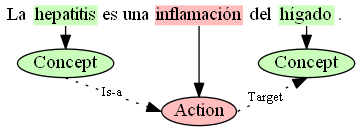
\includegraphics[width=\textwidth]{graphics/annotation_example_is_a.png}
		\caption{Ejemplo de anotación de hiperonimia e hiponimia.}
		\vspace{0.4in}
		\label{fig:annotation_example_is_a}
	\end{subfigure}
	\begin{subfigure}{3.25in}
		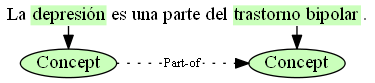
\includegraphics[width=\linewidth]{graphics/annotation_example_part_of.png}
		\caption{Ejemplo de anotación de meronimia y holonimia.}
		\vspace{0.4in}
		\label{fig:annotation_example_part_of}
	\end{subfigure}
	\begin{subfigure}{4.2in}
		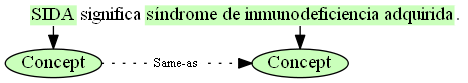
\includegraphics[width=\linewidth]{graphics/annotation_example_same_as.png}
		\caption{Ejemplo de anotación de sinonimia.}
		\vspace{0.4in}
		\label{fig:annotation_example_same_as}
	\end{subfigure}
	\begin{subfigure}{3.9in}
		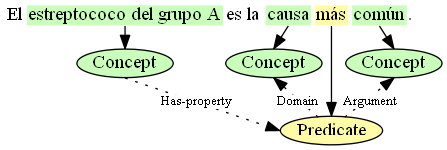
\includegraphics[width=\linewidth]{graphics/annotation_example_has_property.png}
		\caption{Ejemplo de anotación de propiedad.}
		\label{fig:annotation_example_has_property}
	\end{subfigure}
	\caption{Anotación de las relaciones taxonómicas}
\end{figure}

\subsection{Causalidad e implicación}
Las cuatro relaciones semánticas presentadas hasta ahora son útiles para capturar la estructura taxonómica del conocimiento expresado en textos del lenguaje natural. Dos relaciones adicionales son definidas para capturar conexiones lógicas entre conceptos: \textit{causes} y \textit{entails} (en español \textit{causa} e \textit{implica} respectivamente). La relación \textit{causes} es usada para expresar que un evento, identificado en general como un concepto, es una posible causa para otro evento. En la figura \ref{fig:annotation_example_causes} se muestra un ejemplo anotado.

Esta relación indica causalidad, no correlación ni implicación lógica. Por tanto, debe estar declarado con claridad en la oración que hay una conexión de causa directa entre ambos eventos. Además, hay un grado de incertidumbre implicada en la causalidad, lo cual significa que si \guillemot{\texttt{A} \textit{causes} \texttt{B}}, eso no necesariamente implica que cada vez que pase \guillemot{\texttt{A}} sería seguido por \guillemot{\texttt{B}}, ni que en cualquier caso que ocurra \guillemot{\texttt{B}} será a causa de \guillemot{\texttt{A}}.

\begin{figure}[H]
	\centering
	\begin{subfigure}{3.25in}
		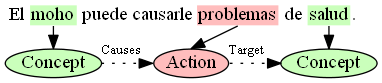
\includegraphics[width=\textwidth]{graphics/annotation_example_causes.png}
		\caption{Ejemplo de anotación de causalidad.}
		\vspace{0.4in}
		\label{fig:annotation_example_causes}
	\end{subfigure}
	\begin{subfigure}{3.9in}
		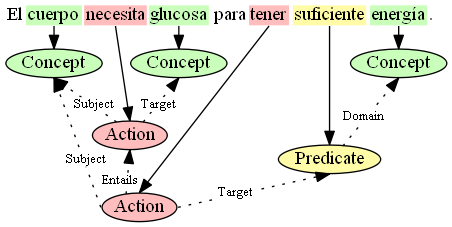
\includegraphics[width=\linewidth]{graphics/annotation_example_entails.png}
		\caption{Ejemplo de anotación de implicación.}
		\label{fig:annotation_example_entails}
	\end{subfigure}
	\caption{Anotación de causalidad e implicación}
\end{figure}

En contraste, la relación \textit{entails} es usada para denotar implicación lógica. En este caso, no es necesario que los eventos estén relacionados por causalidad en lo más mínimo; lo único que debe cumplirse es que cuando la proposición \guillemot{\texttt{A}} es verdadera entonces siempre sucede el caso de que la proposición \guillemot{\texttt{B}} es verdadera. En la figura \ref{fig:annotation_example_entails} puede verse un ejemplo, donde un concepto complejo, en este caso \guillemot{\texttt{tener}} implica \guillemot{\texttt{necesita}}, otro concepto complejo. Desde otro punto de vista, la anotación de esa oración resulta en:

\begin{center}
	\guillemot{$\big($tener [suficiente energía] en el cuerpo$\big)$\\\textit{entails}\\(necesitar glucosa en el cuerpo)}
\end{center}

La anotación de causalidad e implicación evita anotar varias palabras y frases que comparten el mismo significado semántico. Por ejemplo, en la figura \ref{fig:annotation_example_causes} no resulta necesario anotar \guillemot{\texttt{puede causarle}} debido a que el significado correcto está siendo representado por la relación \textit{causes}.

\subsection{Contextualización}
En ocasiones, los conceptos solo participan en determinada relación con precondiciones, como por ejemplo, si dura un período específico de tiempo o solo en una ubicación específica, o con algunas propiedades adicionales.

Un ejemplo es la oración de la figura \ref{fig:annotation_example_in_place}. En esta oración, la anotación \guillemot{\texttt{injerto óseo--transplanta--tejidos}} falla en capturar la semántica completa del mensaje, dado que el \guillemot{\texttt{injerto óseo}} no es necesariamente siempre \guillemot{\texttt{transplantar tejidos}} (según la oración), sino solo en la situación específica en la que el tejido transplantado es de los \guillemot{\texttt{huesos}}. Para resolver estas situaciones, el modelo incluye tres relaciones de contexto: \textit{in-time}, \textit{in-place} y el más general \textit{in-context} (en español \textit{en-tiempo}, \textit{en-lugar} y \textit{en-contexto} respectivamente).

La relación \textit{in-time} restringe un concepto a un instante de tiempo determinado. Además, permite atrapar restricciones más generales siempre que hablen del concepto mientras cumpla determinada condición o durante el tiempo que lo hace. Puede verse un ejemplo en la figura \ref{fig:annotation_example_in_time}.

La relación \textit{in-place} restringe un concepto a un lugar determinado. Además, puede ser visto como la contextualización de la relación \textit{part-of}, en el sentido de que permite plantear un hecho sobre un concepto que es parte de otro. Puede verse un ejemplo en la figura \ref{fig:annotation_example_in_place}.

\begin{figure}[H]
	\centering
	\begin{subfigure}{3.8in}
		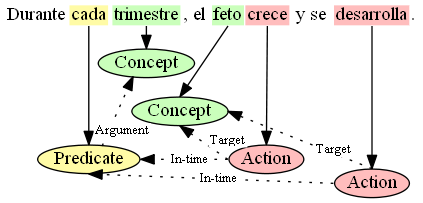
\includegraphics[width=\textwidth]{graphics/annotation_example_in_time.png}
		\caption{Ejemplo de anotación de tiempo.}
		\vspace{0.4in}
		\label{fig:annotation_example_in_time}
	\end{subfigure}
	\begin{subfigure}{3.6in}
		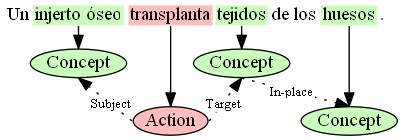
\includegraphics[width=\linewidth]{graphics/annotation_example_in_place.png}
		\caption{Ejemplo de anotación de lugar.}
		\vspace{0.4in}
		\label{fig:annotation_example_in_place}
	\end{subfigure}
	\begin{subfigure}{3.5in}
		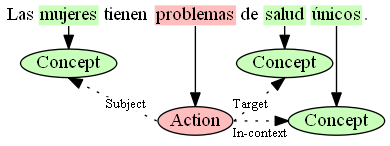
\includegraphics[width=\linewidth]{graphics/annotation_example_in_context.png}
		\caption{Ejemplo de anotación de contexto.}
		\label{fig:annotation_example_in_context}
	\end{subfigure}
	\caption{Anotación de contextualización}
\end{figure}

La relación \textit{in-context} restringe un concepto a condiciones más generales que las descritas anteriormente. Es el contextualizador más general y al igual que el resto, solo debe ser aplicado cuando el contexto habla de un rasgo o valor que puede tener el concepto a contextualizar. Eso implica que el objeto a contextualizar debe tener semántica propia independiente del contexto. De forma general, puede verse como el contextualizador de la relación \textit{has-property}. Un caso de uso particular es en las oraciones imperativas, donde un fragmento como \guillemot{\dots\space \texttt{si X entonces haga Y} \dots} se anotaría como \guillemot{\texttt{Y} \textit{in-context} \texttt{X}}. Puede verse un ejemplo en la figura \ref{fig:annotation_example_in_context}.

La diferencia entre las relaciones de contexto y el resto es que ellas no definen una aserción, sino que son útiles solo para construir conceptos más complejos. Por ejemplo, la anotación \guillemot{\texttt{problemas} \textit{in-context} \texttt{únicos}} no solo significa que las mujeres tienen problemas de salud, sino que además tienen problemas únicos. Es exclusivamente cuando se enlaza con otro concepto, a través de \textit{has-property} u otra relación, que esta construcción toma sentido. Por esta razón, no es correcto intercambiar arbitrariamente \textit{in-context} con \textit{has-property}, ya que una relación \textit{has-property} declara una aserción concreta por sí misma. De igual forma enlazar un concepto sobre el que se ha establecido una relación que no es de contextualización, con otro concepto a través de alguna relación o rol, no indica que dicha relación o rol sea válida solamente para aquellas instancias del concepto que cumplan la propiedad indicada por la relación que no es de contextualización, puesto que estas relaciones, no construyen conceptos complejos que se puedan enlazar.

\subsection{Atributos}
Cuatro atributos booleanos\footnote{HAY QUE PONER ALGO AQUÍ} adicionales pueden ser asociados a cualquier concepto para calificarlo o describirlo aún más. Ellos son: \textit{negated}, \textit{uncertain}, \textit{diminished} y \textit{emphasized} (en español \textit{negación}, \textit{incertidumbre}, \textit{disminución} y \textit{énfasis} respectivamente). Estos atributos son usados para evitar anotar palabras comunes del idioma que son usadas con bastante frecuencia como \textit{no}, \textit{puede}, \textit{poco}, \textit{mucho}, y en su lugar asociar directamente el calificador correspondiente al concepto en sí. Además, los atributos capturan la negación, incertidumbre, disminución o énfasis que se pretendía en la oración aun cuando sea implícito y no indicado explícitamente por otra palabra de la misma. Estos atributos acompañan al concepto que modifican en todas las relaciones en que este participe. En la figura \ref{fig:annotation_examples_attributes} puede verse un ejemplo anotado de cada uno de estos cuatro atributos.

\begin{figure}[H]
	\centering
	\begin{subfigure}{2.4in}
		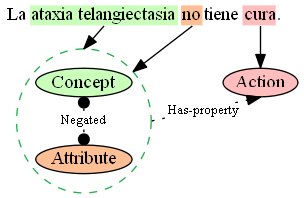
\includegraphics[width=\textwidth]{graphics/annotation_example_attribute_negated.png}
		\caption{Ejemplo de anotación del atributo negación.}
		\vspace{0.3in}
		\label{fig:annotation_example_attribute_negated}
	\end{subfigure}
	\quad
	\begin{subfigure}{2.2in}
		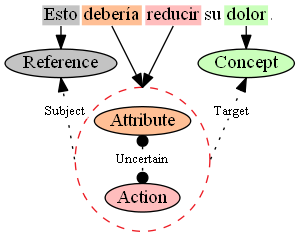
\includegraphics[width=\linewidth]{graphics/annotation_example_attribute_uncertain.png}
		\caption{Ejemplo de anotación del atributo incertidumbre.}
		\vspace{0.3in}
		\label{fig:annotation_example_attribute_uncertain}
	\end{subfigure}
	\begin{subfigure}{4.2in}
		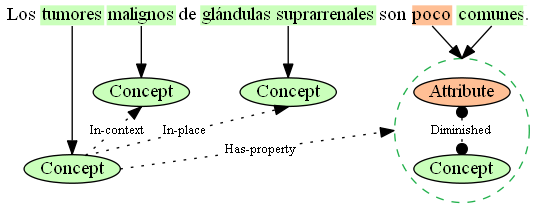
\includegraphics[width=\linewidth]{graphics/annotation_example_attribute_diminished.png}
		\caption{Ejemplo de anotación del atributo disminución.}
		\vspace{0.3in}
		\label{fig:annotation_example_attribute_diminished}
	\end{subfigure}
	\begin{subfigure}{2.3in}
		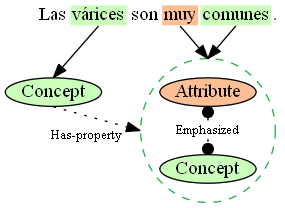
\includegraphics[width=\linewidth]{graphics/annotation_example_attribute_emphasized.png}
		\caption{Ejemplo de anotación del atributo énfasis.}
		\label{fig:annotation_example_attribute_emphasized}
	\end{subfigure}
	\caption{Anotación de los atributos}
	\label{fig:annotation_examples_attributes}
\end{figure}

\section{Análisis del Corpus}
El corpus fue construido a partir de un fichero \textit{XML}\footnote{Siglas en inglés de \textit{e\textbf{X}tensible \textbf{M}arkup \textbf{L}anguage}, un lenguaje de marcado desarrollado por el \textit{World Wide Web Consortium} (W3C).} tomado del sitio web de \textit{Medline} (\textbf{NECESITA REFERENCIAAAAAAAAA}) el $9$ de enero de $2018$, específicamente a las $02:30:31$. \textit{Medline} fue producida y es mantenida por la Biblioteca Nacional de Medicina de los Estados Unidos. Recoge referencias bibliográficas de los artículos publicados en aproximadamente $5,500$ revistas médicas desde $1966$. Actualmente reúne más de $30,000,000$ citas. Cada registro de \textit{Medline} es la referencia bibliográfica de un artículo científico publicado en una revista médica, con los datos bibliográficos básicos de un artículo: título, autores, nombre de la revista, año de publicación, entre otros. Esto permite la recuperación de estas referencias posteriormente en una biblioteca o a través de un \textit{software} específico de recuperación.

\begin{figure}[H]
	\begin{center}
		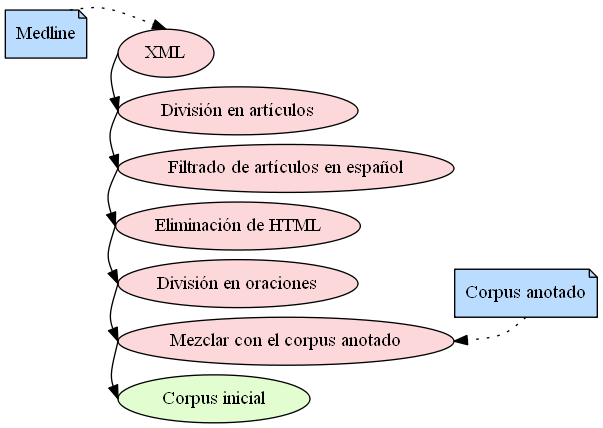
\includegraphics[height=3.6in]{graphics/corpus_processing.png}
		\caption[Esquema del procesamiento inicial del corpus]{Esquema del procesamiento inicial del corpus.}
		\label{fig:corpus_processing}
	\end{center}
\end{figure}

En la figura \ref{fig:corpus_processing} puede verse una representación esquemática del procesamiento inicial que se le hace al corpus de \textit{Medline}, el cual de forma análoga puede aplicarse a otros. En esta investigación solo se trabajará con los artículos en español, estos son procesados para eliminar las marcas específicas de \textit{HTML}\footnote{Siglas en inglés de \textit{\textbf{H}yper\textbf{T}ext \textbf{M}arkup \textbf{L}anguage}, un lenguaje de marcado usado en la elaboración de páginas web.} y ser divididos en oraciones. Luego, las oraciones anotadas son mezcladas con sus respectivos artículos. Potencialmente, un artículo podrá no tener ninguna de sus oraciones anotadas o estar completamente anotado. Las tablas \ref{tab:stats_corpus} y \ref{tab:stats_annotated_corpus} muestran algunas estadísticas acerca de este corpus y de las oraciones anotadas pertenecientes al mismo.

\vspace{-0.02in}
\begin{table}[h!]
	\begin{center}
		\begin{tabular}{lcc}
			\noalign{\hrule height 1pt}\\
			\vspace{-0.35in}\\
			\textbf{Métrica} & \textbf{\textit{Medline}} & \textbf{Anotado}\\
			\hline\\
			\vspace{-0.35in}\\
			Artículos & $1,013$ & $25^*$\\
			\hline\\
			\vspace{-0.35in}\\
			Oraciones & $12,830$ & $999$\\
			Promedio de oraciones por artículo & $\approx13$ & $\approx40$\\
			Menor cantidad de oraciones en un artículo & $2$ & $39$\\
			Artículos con la menor cantidad de oraciones & $9$ & $1$\\
			Mayor cantidad de oraciones en un artículo & $65$ & $40$\\
			Artículos con la mayor cantidad de oraciones & $1$ & $24$\\
			\hline\\
			\vspace{-0.35in}\\
			Palabras & $191,256$ & $14,529$\\
			Promedio de palabras por artículo & $\approx189$ & $\approx581$\\
			Promedio de palabras por oración & $\approx15$ & $\approx15$\\
			Menor cantidad de palabras en un artículo & $33$ & $489$\\
			Artículos con la menor cantidad de palabras & $1$ & $1$\\
			Menor cantidad de palabras en una oración & $1$ & $4$\\
			Oraciones con la menor cantidad de palabras & $87$ & $1$\\
			Mayor cantidad de palabras en un artículo & $1,199$ & $671$\\
			Artículos con la mayor cantidad de palabras & $1$ & $1$\\
			Mayor cantidad de palabras en una oración & $258$ & $46$\\
			Oraciones con la mayor cantidad de palabras & $1$ & $1$\\
			\noalign{\hrule height 1pt}
			\vspace{0in}
		\end{tabular}
		*\small{Esta cifra no son artículos en sí, sino archivos, los cuales pueden contener oraciones de varios artículos.}
		\caption[Estadísticas del corpus tomado de \textit{Medline} y del anotado]{Estadísticas del corpus tomado de \textit{Medline} y del anotado.}
		\label{tab:stats_corpus}
	\end{center}
\end{table}

\begin{table}[h!]
	\begin{center}
		\begin{tabular}{lc}
			\noalign{\hrule height 1pt}\\
			\vspace{-0.35in}\\
			\textbf{Métrica} & \textbf{Total}\\
			\hline\\
			\vspace{-0.35in}\\
			Oraciones & $999$\\
			\hline\\
			\vspace{-0.35in}\\
			Conceptos & $6,324$\\
			\quad \texttt{Concept} & $3,914$\\
			\quad \texttt{Action} & $1,661$\\
			\quad \texttt{Reference} & $213$\\
			\quad \texttt{Predicate} & $536$\\
			\hline\\
			\vspace{-0.35in}\\
			Relaciones & $5,925$\\
			\quad \texttt{Subject} & $859$\\
			\quad \texttt{Target} & $1,688$\\
			\quad \texttt{Domain} & $346$\\
			\quad \texttt{Argument} & $333$\\
			\quad \texttt{Is-a} & $570$\\
			\quad \texttt{Part-of} & $95$\\
			\quad \texttt{Same-as} & $124$\\
			\quad \texttt{Has-property} & $168$\\
			\quad \texttt{Causes} & $381$\\
			\quad \texttt{Entails} & $170$\\
			\quad \texttt{In-time} & $154$\\
			\quad \texttt{In-place} & $384$\\
			\quad \texttt{In-context} & $653$\\
			\hline\\
			\vspace{-0.35in}\\
			Atributos & $559$\\
			\quad \texttt{Negated} & $160$\\
			\quad \texttt{Uncertain} & $262$\\
			\quad \texttt{Diminished} & $17$\\
			\quad \texttt{Emphasized} & $120$\\
			\noalign{\hrule height 1pt}
		\end{tabular}
		\caption[Estadísticas del corpus anotado]{Estadísticas del corpus anotado.}
		\label{tab:stats_annotated_corpus}
	\end{center}
\end{table}

% Finalmente, se obtuvieron 9 956 oraciones,divididas en 41 ficheros según el tema.Usando este conjunto de oraciones, se implementó un proceso de ano-tación  para  etiquetar  manualmente  las  entidades  relevantes  y  relacionessegún el modelo descrito en la sección 2.1. Este proceso de anotación sedescribe en detalle en la sección 2.2. La figura 2.8 ilustra el procesamientorealizado. Luego del proceso de anotación, se obtuvo un total de 1, 045 ora-ciones de dominio médico, divididas en 4 colecciones según se describe acontinuación. La tabla 2.1 resume las estadísticas fundamentales del corpusfinal.La colección de prueba (trial collection) contiene 45 oraciones. Esta colec-ción fue creada antes de comenzar el proceso de anotación, con el propósitode llegar a un consenso común entre los anotadores. La colección de pruebaresume todos los posibles patrones de anotación que aparecen en el texto.A partir de esta colección, una guía de anotación es creada para asistir a losanotadores.Las restantes 1 000 oraciones se dividieron en tres colecciones en el con-texto deleHealth-KD challenge: las colecciones de entrenamiento (training),desarrollo  (development)  y  evaluación  (test),  formadas  por  600,  100  y  300oraciones respectivamente. En la colección de entrenamiento, a diferenciade la edición anterior, las oraciones se unieron en un único fichero en lu-gar de mantenerse separadas en ficheros por tópico. De forma general, lasoraciones en cada colección pertenecen a múltiples temas y están distribui-das aleatoriamente en el fichero. La colección de desarrollo está pensadapara usarse en la selección, validación, y ajuste de hiperparámetros, de los modelos de aprendizaje. A diferencia de la edición anterior, no se busca ga-rantizar un balance entre las colecciones de entrenamiento y evaluación entérminos del número relativo de cada tipo de anotación.


	% proposed solution
	%===================================================================================
% Chapter: Proposed Solution
%===================================================================================
\Chapter{Propuesta de Solución}\label{chapter:proposed_solution}
\vspace{-0.3in}
Esta investigación busca poder expresar un corpus anotado a través de una ontología definida, generando un grafo de conocimiento como resultado. Otro de los objetivos claros, es poder hacer esto de forma automática mediante un algoritmo computacional.
%===================================================================================

\vspace{-0.1in}
\section{Analizador sintáctico}
\vspace{-0.1in}
Primeramente, es necesaria la creación de una herramienta capaz de fragmentar en objetos con significado computacional el contenido de los archivos de anotación escritos con el formato visto en la sección \ref{section:annotation_file_format}.

Dado que en el formato de archivo propuesto contiene una única relación anotada por línea y a su vez, las relaciones tienen su formato de escritura bien definido y sin ambigüedades, llevar a cabo la implementación de este analizador sintáctico es bastante sencillo. Esto puede hacerse a través de expresiones regulares, las cuales son ampliamente usadas y muchos de los lenguajes de programación modernos las incluyen como estructuras integradas.

\vspace{-0.1in}
\section{Modelo ontológico}
\vspace{-0.1in}
La ontología propuesta es de propósito general y basada en el modelo de anotación visto en la sección \ref{section:annotation_structure}. Esto posibilita la continuidad del proceso, partiendo desde documentos escritos en lenguaje natural, hasta la creación de una base de conocimiento a partir de ellos.

Una ontología $O=(C,~R,~A,~Top)$ se define mediante un conjunto no vacío de conceptos $C$, un conjunto de relaciones $R$, un conjunto de axiomas $A$ y $Top$ es el concepto con más alto nivel en la jerarquía. En esta investigación, la ontología propuesta es generada de forma automática, por tanto, las instancias pertenecientes a los conjuntos $C$ y $R$ son generadas de manera automática a medida que se procesa el corpus anotado. Dado que la ontología propuesta no tiene conocimiento previo del dominio, el conjunto $A$ es vacío. A la vez que $Top$ no se sabe a priori qué entidad o instancia de entidad es.

En contraste a definir las instancias de los conjuntos $C$ y $R$, son definidas las clases que serán usadas como base de creación de instancias que pertenecen al conjunto $C$ y las posibles relaciones entre estos, las cuales alimentarán al conjunto $R$ a medida que se va generando la ontología.

Todo concepto en la ontología pertenece a una de las tres clases siguientes: \textit{entidad simple}, \textit{entidad con atributo} o \textit{entidad compuesta}. El significado específico de estas clases, la creación de instancias a partir de ellas y las relaciones que pueden existir entre ellas son explicadas en las secciones siguientes.

\vspace{-0.1in}
\subsection{Clases en la ontología}
\vspace{-0.1in}
Los conceptos usados en la ontología propuesta en esta investigación pertenecen a una de las tres clases siguientes:

\vspace{-0.1in}
\begin{itemize}
	\item[•] Entidad simple: la más sencilla de las clases, no tiene ningún significado especial. En el modelo de la sección \ref{section:annotation_structure} representa un concepto sin haberle aplicado relaciones ni atributos. Cada concepto del modelo de anotación representa una entidad simple. Al ser creada una instancia, la propiedad \guillemot{\texttt{tipo de concepto}} adopta el valor del tipo de concepto específico en el corpus anotado de la palabra o frase correspondiente a la entidad.
	\item[•] Entidad con atributo: está compuesta por una \textit{entidad simple} y uno o más atributos de los mencionados en la sección \ref{section:annotation_structure}. Puede verse como el resultado de haber aplicado todos los atributos pertenecientes a un mismo concepto. Al ser creada una instancia, la propiedad \guillemot{\texttt{tipo de concepto}} adopta el valor del \guillemot{\texttt{tipo de concepto}} de la \textit{entidad simple} que le corresponde.
	\item[•] Entidad compuesta: es el resultado de aplicar las relaciones en el modelo de anotación explicado en la sección \ref{section:annotation_structure}. Está compuesta por la entidad correspondiente al origen y una o más entidades que son objetivos de dicha relación. Al ser creada una instancia, la propiedad \guillemot{\texttt{tipo de concepto}} adopta el valor del \guillemot{\texttt{tipo de concepto}} de la entidad origen que le corresponde.
\end{itemize}

\vspace{-0.1in}
Estas clases contienen, además, dos propiedades; una de ellas es la palabra o fragmento de texto en sí que representa la entidad y la otra es el tipo de concepto al que representan. Esta última propiedad se basa en los cuatro tipos de concepto existentes en el modelo de anotación explicado en la sección \ref{section:annotation_structure}, estos son: \textit{Concept}, \textit{Action}, \textit{Reference} y \textit{Predicate}.

No existen relaciones entre conceptos utilizados en el modelo de anotación y entidades debido a que cada concepto en el corpus anotado pasa a ser una instancia de entidad simple en la ontología. Por tanto, estas relaciones traerían consigo tener nodos inactivos o duplicados, dado que la información estaría duplicada en nodos de tipo concepto y nodos de tipo entidad simple, y además, las relaciones entre estos no aportarían conocimiento nuevo, en cambio, añadirían redundancia a la base de conocimiento.

\vspace{-0.2in}
\subsection{Relaciones en la ontología}
Los tipos de relaciones definidos en la ontología tienen una estrecha relación con los trece tipos de relación vistos en la sección \ref{section:relation_annotation}. Los actores pertenecientes a estas se describen en las secciones siguientes.

\vspace{-0.1in}
\subsubsection{Relación subject}
\vspace{-0.1in}
Puede tener cualquier instancia de entidad como origen y cualquiera como destino. La única restricción es que la entidad de origen debe tener \textit{Action} en la propiedad \guillemot{\texttt{tipo de concepto}}.

\vspace{-0.1in}
\subsubsection{Relación target}
\vspace{-0.1in}
Puede tener cualquier instancia de entidad como origen y cualquiera como destino. La única restricción es que la entidad de origen debe tener \textit{Action} en la propiedad \guillemot{\texttt{tipo de concepto}}.

\vspace{-0.2in}
\subsubsection{Relación domain}
Puede tener cualquier instancia de entidad como origen y cualquiera como destino. La única restricción es que la entidad de origen debe tener \textit{Predicate} en la propiedad \guillemot{\texttt{tipo de concepto}}.

\vspace{-0.1in}
\subsubsection{Relación argument}
\vspace{-0.1in}
Puede tener cualquier instancia de entidad como origen y cualquiera como destino. La única restricción es que la entidad de origen debe tener \textit{Predicate} en la propiedad \guillemot{\texttt{tipo de concepto}}.

\vspace{-0.1in}
\subsubsection{Relación is-a}
\vspace{-0.1in}
Puede tener cualquier instancia de entidad como origen y cualquiera como destino. Relación taxonómica que potencialmente da la posibilidad de descubrir de conocimiento.

\vspace{-0.1in}
\subsubsection{Relación part-of}
\vspace{-0.1in}
Puede tener cualquier instancia de entidad como origen y cualquiera como destino. Relación taxonómica que potencialmente da la posibilidad de descubrir de conocimiento.

\vspace{-0.1in}
\subsubsection{Relación same-as}
\vspace{-0.1in}
Puede tener cualquier instancia de entidad como origen y cualquiera como destino. Relación taxonómica que potencialmente da la posibilidad de descubrir de conocimiento.

\vspace{-0.1in}
\subsubsection{Relación has-property}
\vspace{-0.1in}
Puede tener cualquier instancia de entidad como origen y cualquiera como destino. Relación taxonómica que potencialmente da la posibilidad de descubrir de conocimiento.

\vspace{-0.1in}
\subsubsection{Relación causes}
\vspace{-0.1in}
Puede tener cualquier instancia de entidad como origen y cualquiera como destino. Relación que potencialmente da la posibilidad de descubrir de conocimiento.

\vspace{-0.1in}
\subsubsection{Relación entails}
\vspace{-0.1in}
Puede tener cualquier instancia de entidad como origen y cualquiera como destino. Relación que potencialmente da la posibilidad de descubrir de conocimiento.

\vspace{-0.1in}
\subsubsection{Relación in-time}
\vspace{-0.1in}
Puede tener cualquier instancia de entidad como origen y cualquiera como destino.

\vspace{-0.1in}
\subsubsection{Relación in-place}
\vspace{-0.1in}
Puede tener cualquier instancia de entidad como origen y cualquiera como destino.

\vspace{-0.1in}
\subsubsection{Relación in-context}
\vspace{-0.1in}
Puede tener cualquier instancia de entidad como origen y cualquiera como destino.

La relación directa entre dos instancias de entidades en la base de conocimiento implica la existencia de una relación directa entre ellos en el corpus anotado y viceversa. Por tanto, todo el conocimiento explícito descrito por el corpus será representado por relaciones entre instancias de entidades. Basado en esto, dado un camino $P$ de tamaño dos o más entre dos instancias de entidades $u$ y $v$ en este grafo y además, todas las aristas en $P$ son aristas que posibilitan el descubrimiento de conocimiento, entonces si no existe una arista directamente entre el nodo $u$ y el nodo $v$, el conocimiento inferido por el camino $P$ es válido e implícito en el corpus, por tanto, es conocimiento aprendido.

El proceso de creación de una base de conocimiento específica a partir de la definición de esta ontología es llevado a cabo de forma totalmente automática y no de la manera tradicional, con expertos en el dominio añadiendo relaciones entre clases una tras otra. A la interrogante de en qué orden se llevan a cabo estas relaciones y quiénes participan en ellas se le da respuesta en la próxima sección.

\section{Grafo de conocimiento}
\vspace{-0.1in}
Una vez que se haya analizado sintácticamente todo el corpus, se tendrá la información de las anotaciones en objetos computacionales y será más sencillo el trabajo con estos. En aras de evitar ambigüedades y concentrar el conocimiento para un mejor entendimiento de este y a la misma vez, poder facilitar la tarea de extraerlo de este grafo por un equipo de cómputo, el texto anotado es normalizado. Esto es llevado a cabo teniendo en cuenta las palabras que lo componen, y anotando en su lugar la palabra primitiva de esta. Por ejemplo, la palabra \guillemot{\texttt{sangramiento}} será anotada como \guillemot{\texttt{sangrar}} y la frase \guillemot{\texttt{glóbulos rojos}} como \guillemot{\texttt{glóbulo rojo}}.

Como se vio en la sección \ref{section:annotation_structure}, es necesario aclarar que hay que darle un orden a la creación de las instancias de las clases y las relaciones en este grafo, pues las propias anotaciones de texto y las relaciones tienen un orden implícito entre ellas. Por ejemplo, en la propia figura \ref{fig:annotation_example_composing_concepts}, se debe procesar primero el rol ejercido por \guillemot{\texttt{problemas}} y por \guillemot{\texttt{cumpla}} antes de poder procesar \guillemot{\texttt{impiden}}; de lo contrario, el conocimiento descrito por \guillemot{\texttt{impiden}} quedaría incompleto o mal representado.

\vspace{-0.1in}
\subsection{Orden topológico}
\vspace{-0.1in}
El orden establecido por el modelo de anotación visto en el capítulo \ref{chapter:annotation_model} es un orden topológico. Para ello se tiene en cuenta el siguiente orden:

\begin{enumerate}\label{enum:knowledge_graph_build_order}
	\vspace{-0.1in}
	\item Texto: son procesados primero los conceptos del corpus anotado, los cuales son convertidos a instancias de \textit{entidad simple}.
	\vspace{-0.1in}
	\item Atributos: luego son procesados aquellos conceptos que son modificados por atributos en el corpus anotado, los cuales son convertidos a instancias de \textit{entidad con atributo}, usando como base la \textit{entidad simple} correspondiente a dicho concepto.
	\vspace{-0.1in}
	\item Relaciones de acción, predicado y contextualización: luego se procesan estas relaciones, las cuales son representadas por instancias de \textit{entidad compuesta}. Además, para cada concepto que actúa en ellas, se busca su correspondiente instancia de entidad perteneciente al grafo de conocimiento.
	\vspace{-0.1in}
	\item Relaciones taxonómicas y de causa e implicación: por último son añadidas las relaciones que posibilitan el descubrimiento ímplicito en el corpus. Estas no representan nodos en el grafo, y de igual forma que en el paso anterior, para cada concepto que actúa en ellas, se busca su correspondiente instancia de entidad perteneciente al grafo de conocimiento.
\end{enumerate}

Una vez divididas las relaciones en estos tres grupos, estas son asociadas nuevamente, esta vez teniendo en cuenta la parte izquierda de cada una de ellas (\texttt{Arg1} en el archivo de anotación). Una instancia de clase es creada por cada una de estas agrupaciones resultantes, además, una instancia creada en un nivel más avanzado, teniendo en cuenta el orden visto anteriormente, representa una mayor cantidad de información y al mismo tiempo, información más específica respecto a su instancia asociada en niveles anteriores.

\subsection{Ejemplos de generación automática de ontologías}
A continuación se presentan dos ejemplos de la creación de una base de conocimiento a partir de un corpus anotado. En ambos casos, el corpus solo contiene un documento, y este está compuesto por una sola oración. La flecha que puede haber en algunas líneas de los documentos de ejemplo, significa que esta en el mismo es muy larga para ser mostrada en una única línea en este escrito y se continuará escribiendo debajo. En estos ejemplos, las palabras o frases no son normalizadas para un mejor entendimiento en lenguaje natural y además, porque hay varias formas, métodos y decisiones de cómo normalizar palabras o frases.

\subsubsection{Primer ejemplo}
En la figura \ref{fig:text_document1} puede verse el documento de texto de prueba empleado en el primer ejemplo. A su vez, en la figura \ref{fig:annotated_document1} se ve el documento anotado asociado a este. Como puede apreciarse, se siguieron los convenios establecidos en la sección \ref{section:annotation_conventions}. Por último, la base de conocimiento generada para este ejemplo puede verse en la figura \ref{fig:knowledge_graph1.3}.

\begin{annexample}
	[backgroundcolor=black!5]
	{4.9in}
	{fig:text_document1}
	{Ejemplo 1: documento \doublequote{\texttt{desmayo.txt}}}
	{Ejemplo 1: documento \doublequote{\texttt{desmayo.txt}}.}
	El desmayo (o síncope) es una pérdida temporal de la {\scriptsize $\hookrightarrow$}\\
	conciencia.
\end{annexample}

\begin{annexample}
	[backgroundcolor=cyan!13]
	{4.9in}
	{fig:annotated_document1}
	{Ejemplo 1: documento \doublequote{\texttt{desmayo.ann}}}
	{Ejemplo 1: documento \doublequote{\texttt{desmayo.ann}}.}
	\# Sentence 1: El desmayo (o síncope) es una pérdida {\scriptsize $\hookrightarrow$}\\
	temporal de la conciencia.\\
	\# Keyphrases\\
	T1\space\space Concept 3 10\space\space\space\space desmayo\\
	T2\space\space Concept 14 21\space\space\space síncope\\
	T3\space\space Action 30 37\space\space\space\space pérdida\\
	T4\space\space Concept 38 46\space\space\space temporal\\
	T5\space\space Concept 53 63\space\space\space conciencia\\
	\# Relations\\
	R1\space\space is-a Arg1:T1 Arg2:T3\\
	R2\space\space in-context Arg1:T3 Arg2:T4\\
	R3\space\space target Arg1:T3 Arg2:T5\\
	\textasteriskcentered\space\space\space same-as T1 T2
\end{annexample}

Siguiendo el orden topológico establecido \hyperref[enum:knowledge_graph_build_order]{anteriormente}, se puede ver en la figura \ref{fig:knowledge_graph1.1} el grafo de conocimiento resultante luego de realizado el punto $1$, donde cada concepto del corpus anotado es transformado en una instancia de entidad simple en la base de conocimiento.

\begin{figure}[H]
	\begin{center}
		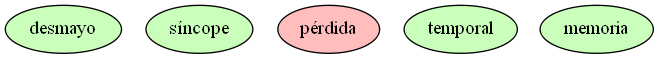
\includegraphics[width=4.5in]{graphics/knowledge_graph_example1_1.png}
		\caption[Ejemplo 1: grafo de conocimiento luego de realizado el punto 1]{Ejemplo 1: grafo de conocimiento luego de realizado el punto 1.}
		\label{fig:knowledge_graph1.1}
	\end{center}
\end{figure}

\vspace{-0.25in}
En el punto $2$ del orden topológico no puede hacerse nada en este corpus, pues no hay atributos, por tanto, el grafo de conocimiento quedará idéntico. Para el punto $3$ son usadas las relaciones \texttt{R2} y \texttt{R3}, resultando:

\vspace{-0.05in}
\begin{figure}[H]
	\begin{center}
		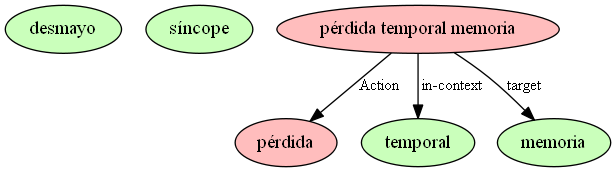
\includegraphics[width=4.7in]{graphics/knowledge_graph_example1_2.png}
		\caption[Ejemplo 1: grafo de conocimiento luego de realizado el punto 3]{Ejemplo 1: grafo de conocimiento luego de realizado el punto 3.}
		\label{fig:knowledge_graph1.2}
	\end{center}
\end{figure}

\vspace{-0.25in}
Para el punto $4$ son usadas las relaciones que potencialmente posibilitan el conocimiento ímplicito en el corpus. En este caso son: \texttt{R1} y \texttt{\textasteriskcentered}. Resultando:

\vspace{-0.05in}
\begin{figure}[H]
	\begin{center}
		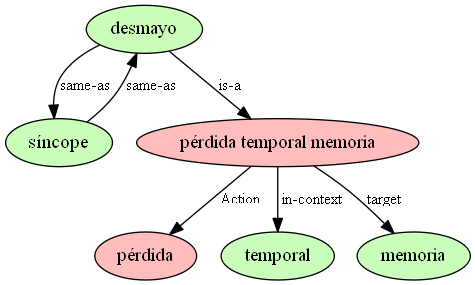
\includegraphics[width=3.6in]{graphics/knowledge_graph_example1_3.png}
		\caption[Ejemplo 1: grafo de conocimiento luego de realizado el punto 4]{Ejemplo 1: grafo de conocimiento luego de realizado el punto 4.}
		\label{fig:knowledge_graph1.3}
	\end{center}
\end{figure}

El ejemplo anterior es sencillo, pero aun así, puede descubrirse conocimiento implícito. Se infiere que \guillemot{\texttt{síncope} \textit{is-a} \texttt{pérdida temporal memoria}}.

\vspace{-0.1in}
\subsubsection{Segundo ejemplo}
\vspace{-0.1in}
En la figura \ref{fig:text_document2} puede verse el documento de texto de prueba empleado en el segundo ejemplo. A su vez, en la figura \ref{fig:annotated_document2} se ve el documento anotado asociado a este. Como puede apreciarse, en este documento también se siguieron los convenios establecidos en la sección \ref{section:annotation_conventions}. Por último, la base de conocimiento generada para este ejemplo puede verse en la figura \ref{fig:knowledge_graph2.4}.

\vspace{-0.1in}
\begin{annexample}
[backgroundcolor=black!5]
{\textwidth}
{fig:text_document2}
{Ejemplo 2: documento \doublequote{\texttt{higiene.txt}}}
{Ejemplo 2: documento \doublequote{\texttt{higiene.txt}}.}
	Las buenas prácticas de higiene, incluyendo lavarse las {\scriptsize $\hookrightarrow$}\\
	manos correctamente, pueden evitar infecciones.
\end{annexample}

\vspace{-0.2in}
\begin{annexample}
[backgroundcolor=cyan!13]
{\textwidth}
{fig:annotated_document2}
{Ejemplo 2: documento \doublequote{\texttt{higiene.ann}}}
{Ejemplo 2: documento \doublequote{\texttt{higiene.ann}}.}
	\# Sentence 1: Las buenas prácticas de higiene, incluyendo {\scriptsize $\hookrightarrow$}\\
	lavarse las manos correctamente, pueden evitar infecciones.\\
	\# Keyphrases\\
	T1\space\space Concept 4 10\space\space\space\space buenas\\
	T2\space\space Predicate 11 20 prácticas\\
	T3\space\space Concept 24 31\space\space\space higiene\\
	T4\space\space Action 44 51\space\space\space\space lavarse\\
	T5\space\space Concept 56 61\space\space\space manos\\
	T6\space\space Concept 62 75\space\space\space correctamente\\
	T7\space\space Action 84 90\space\space\space\space evitar\\
	T8\space\space Concept 91 102\space\space infecciones\\
	\# Relations\\
	R1\space\space in-context Arg1:T2 Arg2:T1\\
	R2\space\space domain Arg1:T2 Arg2:T3\\
	R3\space\space causes Arg1:T2 Arg2:T7\\
	R4\space\space is-a Arg1:T4 Arg2:T2\\
	R5\space\space target Arg1:T4 Arg2:T5\\
	R6\space\space in-context Arg1:T4 Arg2:T6\\
	R7\space\space target Arg1:T7 Arg2:T8\\
	\# Attributes\\
	A1\space\space Uncertain T7
\end{annexample}

Una vez más, siguiendo el orden establecido \hyperref[enum:knowledge_graph_build_order]{anteriormente}, se puede ver en la figura \ref{fig:knowledge_graph2.1} el grafo de conocimiento resultante luego de realizado el punto $1$, representando cada concepto del corpus anotado como una instancia de entidad simple.

\begin{figure}[H]
	\begin{center}
		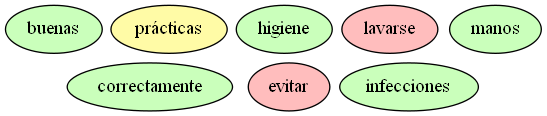
\includegraphics[width=4.2in]{graphics/knowledge_graph_example2_1.png}
		\caption[Ejemplo 2: grafo de conocimiento luego de realizado el punto 1]{Ejemplo 2: grafo de conocimiento luego de realizado el punto 1.}
		\label{fig:knowledge_graph2.1}
	\end{center}
\end{figure}

\vspace{-0.2in}
Dándole solución al punto $2$, los atributos del corpus anotado son representados como una instancia de entidad con atributo. Resultando:
\begin{figure}[H]
	\begin{center}
		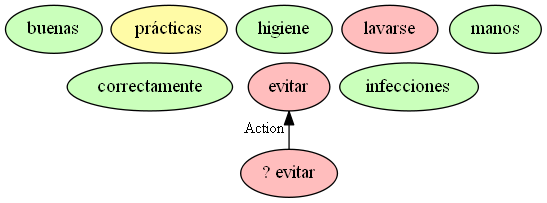
\includegraphics[width=4.2in]{graphics/knowledge_graph_example2_2.png}
		\caption[Ejemplo 2: grafo de conocimiento luego de realizado el punto 2]{Ejemplo 2: grafo de conocimiento luego de realizado el punto 2.}
		\label{fig:knowledge_graph2.2}
	\end{center}
\end{figure}

\vspace{-0.2in}
En aras de completar el punto $3$, las relaciones de acción, predicado y contextualización toman lugar. Resultando:
\begin{figure}[H]
	\begin{center}
		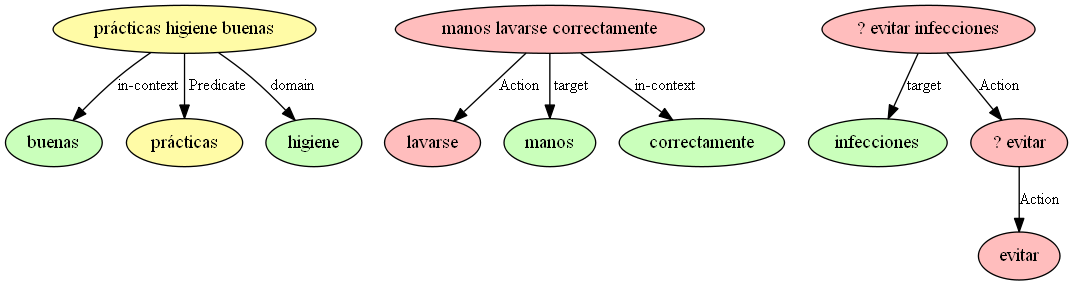
\includegraphics[width=\textwidth]{graphics/knowledge_graph_example2_3.png}
		\caption[Ejemplo 2: grafo de conocimiento luego de realizado el punto 3]{Ejemplo 2: grafo de conocimiento luego de realizado el punto 3.}
		\label{fig:knowledge_graph2.3}
	\end{center}
\end{figure}

Finalmente, al llevar a cabo el punto $4$, son agregadas las relaciones que posibilitan el descubrimiento de conocimiento implícito en el corpus. El grafo de conocimiento resultante de este ejemplo es:
\begin{figure}[H]
	\begin{center}
		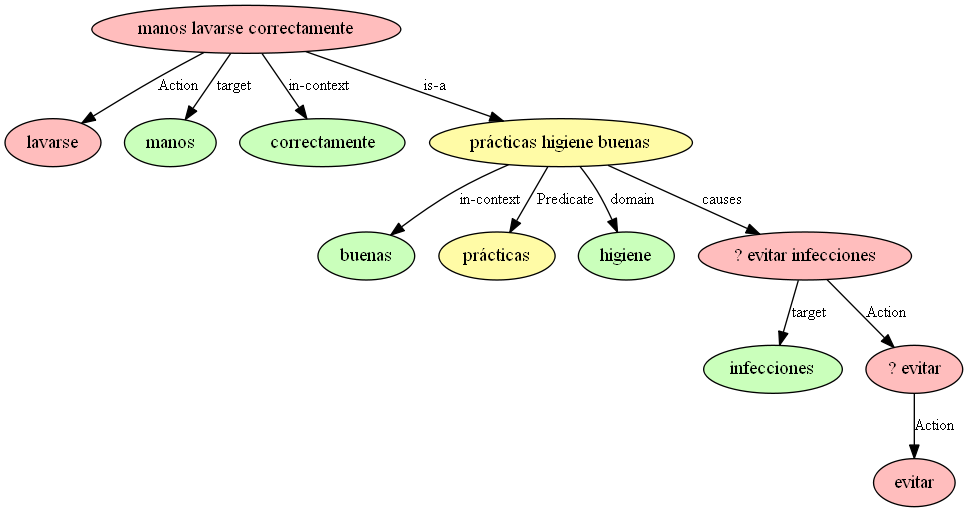
\includegraphics[width=\textwidth]{graphics/knowledge_graph_example2_4.png}
		\caption[Ejemplo 2: grafo de conocimiento luego de realizado el punto 4]{Ejemplo 2: grafo de conocimiento luego de realizado el punto 4.}
		\label{fig:knowledge_graph2.4}
	\end{center}
\end{figure}

Aunque el ejemplo anterior es sencillo, de igual forma que en el primer ejemplo, se puede descubrir conocimiento implícito. En esta ocasión se infiere que \guillemot{\texttt{manos lavarse correctamente} \textit{causes} \texttt{? evitar infecciones}}. Este conocimiento es traducido al lenguaje natural como \doublequote{lavarse las manos correctamente causa que puedan evitarse infecciones}.

Como pudo apreciarse en el ejemplo anterior, se optó por mostrar los atributos en el grafo a través de caracteres en vez de la palabra en sí. Son usados los siguientes caracteres:
\begin{itemize}
	\item[$\lnot$] negación
	\item[?] incertidumbre
	\item[$\downarrow$] disminución
	\item[$\uparrow$] énfasis
\end{itemize}

\subsection{Resumen del algoritmo}\label{section:ontology_construction}
Para llevar a cabo el punto $1$ en el orden previamente expuesto, se crea una \textit{entidad simple} por cada concepto existente en el documento de anotación. Esto sienta las bases para la posterior realización y correctitud del algoritmo expuesto en la sección anterior.

Para satisfacer lo propuesto en el punto $2$, cumplen un papel protagónico las entidades de los conceptos que tienen atributos asociados. En este punto, todas estas son del tipo \textit{entidad simple} y cada una de ellas se une con todos sus respectivos atributos, formando una \textit{entidad con atributo}.

En el paso $3$ tienen lugar algunas de las relaciones. Cada una de ellas conforma una \textit{entidad compuesta}. Esta nueva instancia se relaciona con los conceptos de las partes derecha de dichas relaciones, ahora representados en alguno de los tres tipos de clases de esta ontología, a través del tipo de relación. A la vez que se relaciona con la parte izquierda de estas por medio del tipo de entidad que sean.

El paso $4$ no crea instancias nuevas, solo establece la relación entre dos instancias creadas previamente en el grafo, aportando así conocimiento al mismo.

\section{Alineación de términos}
En el marco del ámbito social y mundial en que fue hecha esta investigación y por motivos principalmente de recursos, no pudo llevarse a cabo una investigación completa de este tema. En su lugar, se realizó un enfoque básico usando lematización y alineación de términos. Esto se logra por medio de la normalización de palabras o frases usadas como conceptos en el corpus anotado, una vez vayan a ser representados en la base de conocimiento. Además, se ofrecen estadísticas y resultados en este acercamiento al problema.

Con el paso del tiempo, la resolución de correferencias pasó de estar plenamente involucrado con este estudio a ser una recomendación para el futuro. Este problema es un primer acercamiento que mejorará la calidad y cantidad de conocimiento implícito descubierto, a la vez de mejorar los resultados alcanzados en esta investigación. De esta manera se dejan abiertas las puertas para la continuación y mejora de lo que aquí se presenta.

	% results
	%===================================================================================
% Chapter: Analysis of Results
%===================================================================================
\chapter{Análisis de Resultados}\label{chapter:analysis-of-results}
%===================================================================================
El esquema de anotación y el modelo ontológico presentado en este trabajo, y por tanto el grafo de conocimiento generado a partir de ellos, tienen como objetivo fundamental asistir en el desarrollo de sistemas de descubrimiento de conocimiento en documentos escritos en lenguaje natural.

En este capítulo, se presenta el marco experimental diseñado para comprobar la efectividad del esquema de anotación y el modelo ontológico descrito en el capítulo \ref{chapter:annotation_model} y de la propuesta de solución presentada en el capítulo \ref{chapter:proposed-solution}.

\section{Marco experimental}
En esta investigación solo se trabajará con los artículos del corpus de \textit{Medline} en español, estos son procesados para eliminar las marcas específicas de \textit{HTML}\footnote{Siglas en inglés de \textit{\textbf{H}yper\textbf{T}ext \textbf{M}arkup \textbf{L}anguage}, un lenguaje de marcado usado en la elaboración de páginas web.} y ser divididos en oraciones. Luego, las oraciones anotadas son mezcladas con sus respectivos artículos. Potencialmente, un artículo podrá no tener ninguna de sus oraciones anotadas o estar completamente anotado. Las tablas \ref{tab:stats_corpus} y \ref{tab:stats_annotated_corpus} muestran algunas estadísticas acerca de este corpus y de las oraciones anotadas pertenecientes al mismo.

Estos resultados son extraídos usando \textit{python} como lenguaje de programación y los paquetes \textit{nltk} y \textit{spacy} para el procesamiento del lenguaje natural.

\begin{table}[H]
	\begin{center}
		\begin{tabular}{lccc}
			\noalign{\hrule height 1pt}\\
			\vspace{-0.35in}\\
			\textbf{Métrica} & \textbf{\textit{Medline}} & \textbf{Anotado} & \textbf{\% anotado}\\
			\hline\\
			\vspace{-0.35in}\\
			Artículos & $1,013$ & $25^*$ & $\approx2.47$\\
			\hline\\
			\vspace{-0.35in}\\
			Oraciones & $12,830$ & $999$ & $\approx7.79$\\
			Promedio de oraciones por artículo & $\approx13$ & $\approx40$ & $\approx307.69$\\
			Menor cantidad de oraciones en un artículo & $2$ & $39$ & $1,950$\\
			Artículos con la menor cantidad de oraciones & $9$ & $1$ & $\approx11.11$\\
			Mayor cantidad de oraciones en un artículo & $65$ & $40$ & $\approx61.54$\\
			Artículos con la mayor cantidad de oraciones & $1$ & $24$ & $2,400$\\
			\hline\\
			\vspace{-0.35in}\\
			Palabras & $191,256$ & $14,529$ & $\approx7.6$\\
			Promedio de palabras por artículo & $\approx189$ & $\approx581$ & $\approx307.41$\\
			Promedio de palabras por oración & $\approx15$ & $\approx15$ & $100$\\
			Menor cantidad de palabras en un artículo & $33$ & $489$ & $\approx1,481.82$\\
			Artículos con la menor cantidad de palabras & $1$ & $1$ & $100$\\
			Menor cantidad de palabras en una oración & $1$ & $4$ & $400$\\
			Oraciones con la menor cantidad de palabras & $87$ & $1$ & $\approx1.15$\\
			Mayor cantidad de palabras en un artículo & $1,199$ & $671$ & $\approx55.96$\\
			Artículos con la mayor cantidad de palabras & $1$ & $1$ & $100$\\
			Mayor cantidad de palabras en una oración & $258$ & $46$ & $\approx17.83$\\
			Oraciones con la mayor cantidad de palabras & $1$ & $1$ & $100$\\
			\noalign{\hrule height 1pt}\\
		\end{tabular}

		\vspace{-0.1in}
		*\small{Esta cifra no son artículos en sí, sino archivos, los cuales pueden contener oraciones de varios artículos.}
		\caption[Estadísticas del corpus tomado de \textit{Medline} y del anotado]{Estadísticas del corpus tomado de \textit{Medline} y del anotado.}
		\label{tab:stats_corpus}
	\end{center}
\end{table}

\begin{table}[H]
	\begin{center}
		\begin{tabular}{lcc}
			\noalign{\hrule height 1pt}\\
			\vspace{-0.35in}\\
			\textbf{Métrica} & \textbf{Total}\\
			\hline\\
			\vspace{-0.35in}\\
			Oraciones & $999$\\
			\hline\\
			\vspace{-0.35in}\\
			Conceptos & $6,324$ & \% conceptos\\
			\quad \texttt{Concept} & $3,914$ & $\approx61.89$\\
			\quad \texttt{Action} & $1,661$ & $\approx26.27$\\
			\quad \texttt{Reference} & $213$ & $\approx3.37$\\
			\quad \texttt{Predicate} & $536$ & $\approx8.47$\\
			\hline\\
			\vspace{-0.35in}\\
			Relaciones & $5,925$ & \% relaciones\\
			\quad \texttt{Subject} & $859$ & $\approx14.5$\\
			\quad \texttt{Target} & $1,688$ & $\approx28.49$\\
			\quad \texttt{Domain} & $346$ & $\approx5.84$\\
			\quad \texttt{Argument} & $333$ & $\approx5.62$\\
			\quad \texttt{Is-a} & $570$ & $\approx9.62$\\
			\quad \texttt{Part-of} & $95$ & $\approx1.6$\\
			\quad \texttt{Same-as} & $124$ & $\approx2.09$\\
			\quad \texttt{Has-property} & $168$ & $\approx2.84$\\
			\quad \texttt{Causes} & $381$ & $\approx6.43$\\
			\quad \texttt{Entails} & $170$ & $\approx2.87$\\
			\quad \texttt{In-time} & $154$ & $\approx2.6$\\
			\quad \texttt{In-place} & $384$ & $\approx6.48$\\
			\quad \texttt{In-context} & $653$ & $\approx11.02$\\
			\hline\\
			\vspace{-0.35in}\\
			Atributos & $559$ & \% atributos\\
			\quad \texttt{Negated} & $160$ & $\approx28.62$\\
			\quad \texttt{Uncertain} & $262$ & $\approx46.87$\\
			\quad \texttt{Diminished} & $17$ & $\approx3.04$\\
			\quad \texttt{Emphasized} & $120$ & $\approx21.47$\\
			\noalign{\hrule height 1pt}
		\end{tabular}
		\caption[Estadísticas del corpus anotado]{Estadísticas del corpus anotado.}
		\label{tab:stats_annotated_corpus}
	\end{center}
\end{table}

\section{Resultados computacionales}
En la figura \ref{fig:out_degree_all_nodes} se evidencia una relación entre el grado de salida de los nodos y la cantidad de estos que tienen un grado específico. Esto representa la cantidad de relaciones como las explicadas en la sección \ref{section:relation_annotation} en las que el nodo es parte izquierda (referenciado a través de \texttt{Arg1}).
\begin{figure}[H]
	\begin{center}
		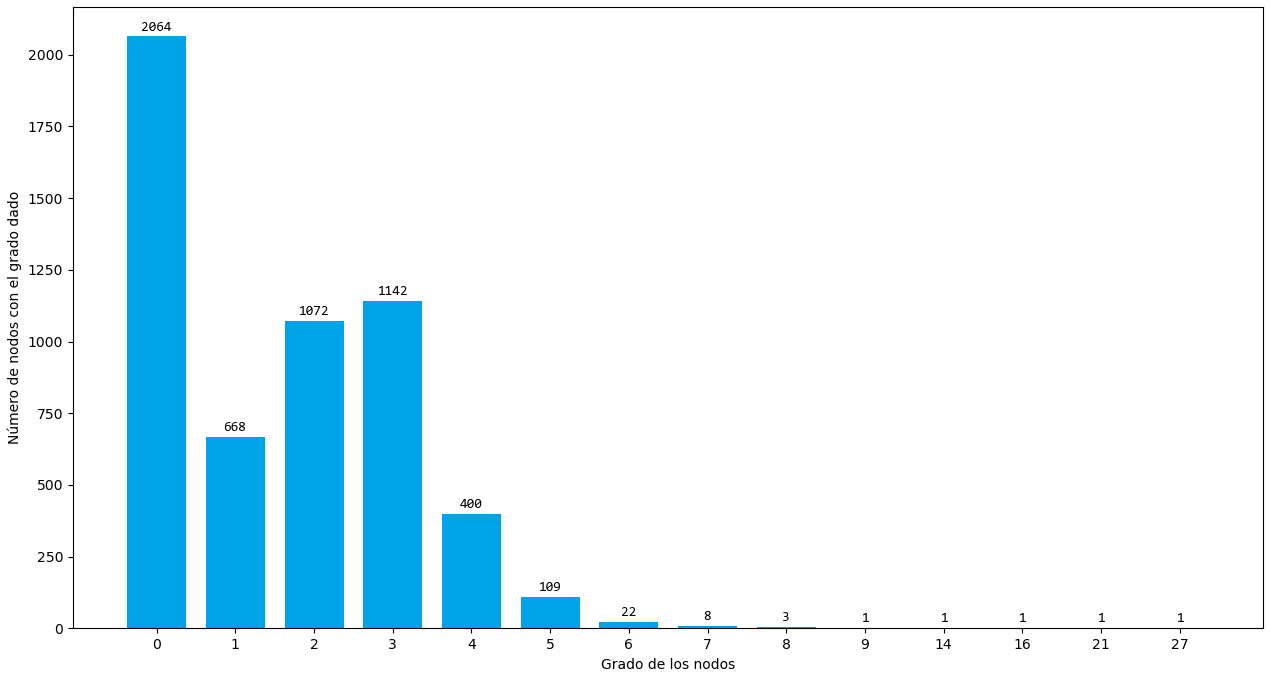
\includegraphics[width=\textwidth]{graphics/degree1.png}
		\caption[Grado de salida de los nodos del grafo]{Grado de salida de los nodos del grafo.}
		\label{fig:out_degree_all_nodes}
	\end{center}
\end{figure}

En la figura \ref{fig:in_degree_all_nodes} se evidencia una relación entre el grado de salida de los nodos y la cantidad de estos que tienen un grado específico. Esto representa la cantidad de relaciones como las explicadas en la sección \ref{section:relation_annotation} en las que el nodo es parte derecha (referenciado a través de \texttt{Arg2}).
\begin{figure}[H]
	\begin{center}
		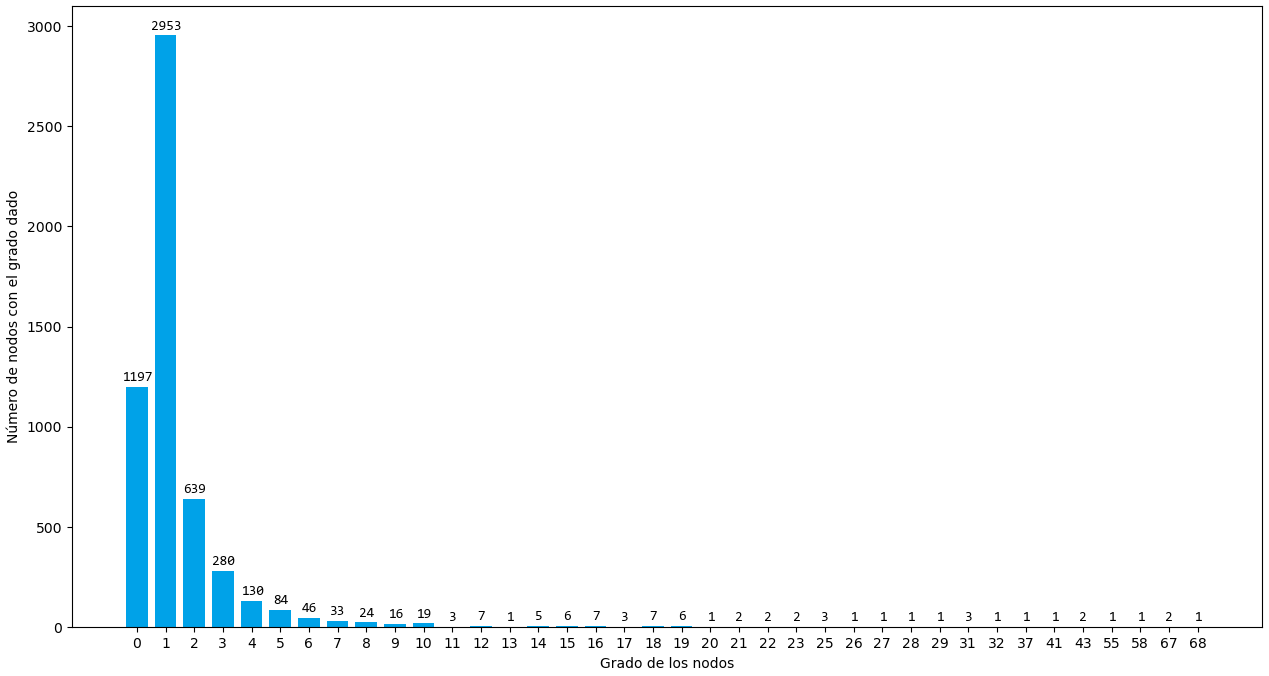
\includegraphics[width=\textwidth]{graphics/degree2.png}
		\caption[Grado de entrada de los nodos del grafo]{Grado de entrada de los nodos del grafo.}
		\label{fig:in_degree_all_nodes}
	\end{center}
\end{figure}

En la figura \ref{fig:out_degree_nodes_by_rol} se evidencia una relación entre el grado de salida de los nodos y la cantidad de estos que tienen un grado específico, pero esta vez agrupados por su rol semántico. Esto representa la cantidad de relaciones como las explicadas en la sección \ref{section:relation_annotation} en las que el nodo es parte izquierda (referenciado a través de \texttt{Arg1}).
\begin{figure}[H]
	\begin{center}
		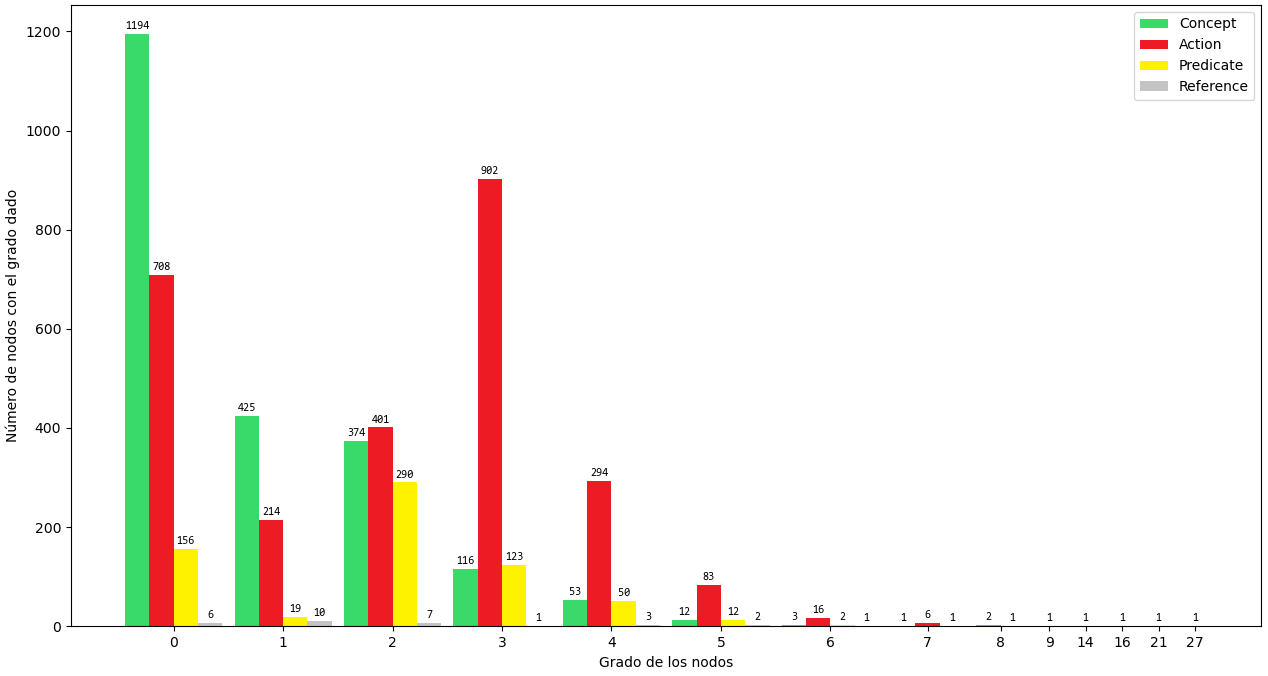
\includegraphics[width=\textwidth]{graphics/degree3.png}
		\caption[Grado de salida de los nodos del grafo por rol]{Grado de salida de los nodos del grafo por rol.}
		\label{fig:out_degree_nodes_by_rol}
	\end{center}
\end{figure}

En la figura \ref{fig:in_degree_nodes_by_rol} se evidencia una relación entre el grado de salida de los nodos y la cantidad de estos que tienen un grado específico, pero esta vez agrupados por su rol semántico. Esto representa la cantidad de relaciones como las explicadas en la sección \ref{section:relation_annotation} en las que el nodo es parte derecha (referenciado a través de \texttt{Arg2}).
\begin{figure}[H]
	\begin{center}
		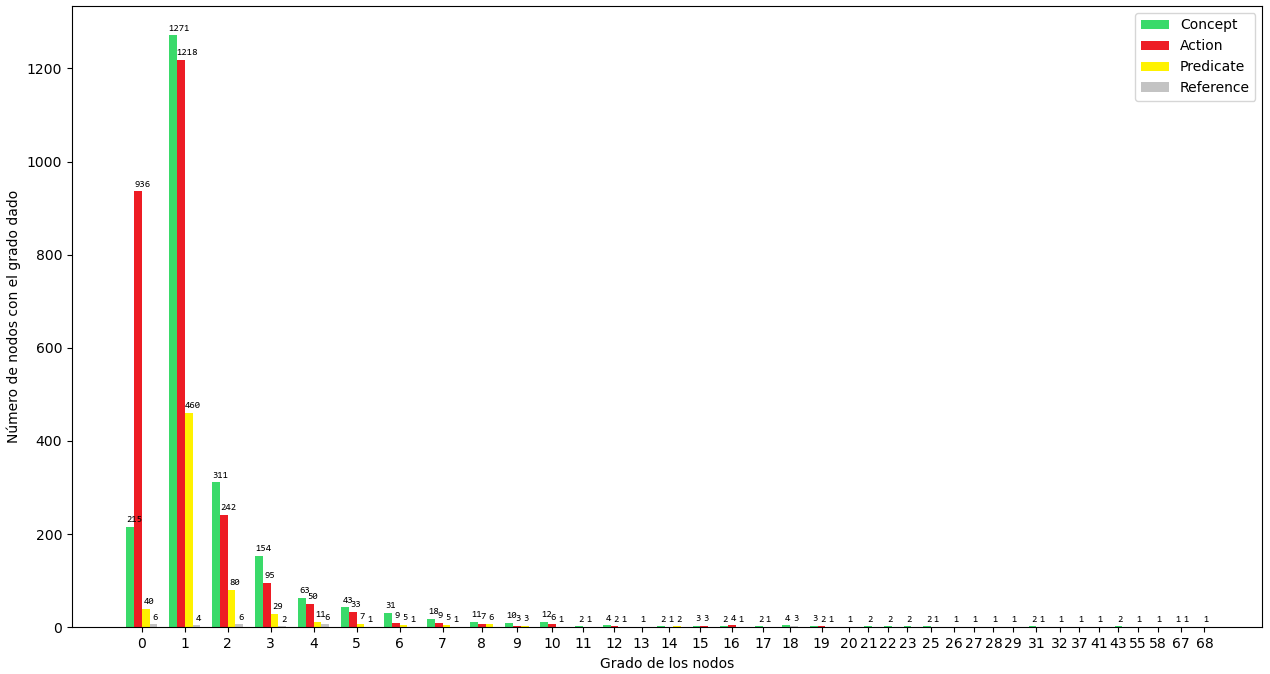
\includegraphics[width=\textwidth]{graphics/degree4.png}
		\caption[Grado de entrada de los nodos del grafo por rol]{Grado de entrada de los nodos del grafo por rol.}
		\label{fig:in_degree_nodes_by_rol}
	\end{center}
\end{figure}

En la tabla \ref{tab:knowledge_graph_stats} se aprecia la cantidad de nodos y aristas según su tipo y a la misma vez se comparan los resultados obtenidos sin normalizar y normalizando las palabras respectivamente. La última columna representa el porcentaje de disminución en cada fila luego de normalizar.
%Esto posibilita una mayor coincidencia de las palabras o frases y por ende, es ideal para una mejor representación y extracción del conocimiento.
\begin{table}[H]
	\begin{center}
		\begin{tabular}{lccc}
			\noalign{\hrule height 1pt}\\
			\vspace{-0.35in}\\
			\textbf{Métrica} & \textbf{Sin normalizar} & \textbf{Normalizando} & \textbf{\% disminuido}\\
			\hline\\
			\vspace{-0.35in}\\
			Conceptos & $5,493$ & $4,935$ & $\approx10.16$\\
			\quad \texttt{Concept} & $2,181$ & $1,969$ & $\approx9.72$\\
			\quad \texttt{Action} & $2,625$ & $2,335$ & $\approx11.05$\\
			\quad \texttt{Reference} & $35$ & $21$ & $40$\\
			\quad \texttt{Predicate} & $652$ & $610$ & $\approx6.44$\\
			\hline\\
			\vspace{-0.35in}\\
			Relaciones & $8,682$ & $8,623$ & $\approx0.68$\\
			\quad \texttt{Concept} & $530$ & $525$ & $\approx0.94$\\
			\quad \texttt{Reference} & $9$ & $9$ & $0$\\
			\quad \texttt{Action} & $1,902$ & $1,875$ & $\approx1.42$\\
			\quad \texttt{Subject} & $923$ & $922$ & $\approx0.11$\\
			\quad \texttt{Target} & $1,572$ & $1,568$ & $\approx0.25$\\
			\quad \texttt{Predicate} & $501$ & $496$ & $\approx1$\\
			\quad \texttt{Domain} & $298$ & $296$ & $\approx0.67$\\
			\quad \texttt{Argument} & $308$ & $307$ & $\approx0.32$\\
			\quad \texttt{Is-a} & $492$ & $481$ & $\approx2.24$\\
			\quad \texttt{Part-of} & $89$ & $89$ & $0$\\
			\quad \texttt{Same-as} & $231$ & $231$ & $0$\\
			\quad \texttt{Has-property} & $143$ & $143$ & $0$\\
			\quad \texttt{Causes} & $360$ & $360$ & $0$\\
			\quad \texttt{Entails} & $200$ & $199$ & $0.5$\\
			\quad \texttt{In-time} & $154$ & $154$ & $0$\\
			\quad \texttt{In-place} & $361$ & $360$ & $\approx0.28$\\
			\quad \texttt{In-context} & $609$ & $608$ & $\approx0.16$\\
			\hline\\
			\vspace{-0.35in}\\
			Atributos & $359$ & $329$ & $\approx8.36$\\
			\quad \texttt{Negated} & $111$ & $94$ & $\approx15.32$\\
			\quad \texttt{Uncertain} & $150$ & $141$ & $6$\\
			\quad \texttt{Diminished} & $83$ & $80$ & $\approx3.61$\\
			\quad \texttt{Emphasized} & $15$ & $14$ & $\approx6.67$\\
			\noalign{\hrule height 1pt}
		\end{tabular}
		\caption[Estadísticas del grafo de conocimiento]{Estadísticas del grafo de conocimiento.}
		\label{tab:knowledge_graph_stats}
	\end{center}
\end{table}

Como se ha podido observar anteriormente, una de las principales funciones de las ontologías y los grafos de conocimiento es la extracción de conocimiento que no está representado explícitamente en el corpus. Un ejemplo de ello es:

\begin{table}[H]
	\begin{center}
		\begin{tabular}{cc}
			\noalign{\hrule height 1pt}\\
			\vspace{-0.35in}\\
			\textbf{Documento} & \textbf{Relación explícita}\\
			\hline\\
			\vspace{-0.35in}\\
			\texttt{cirugía.ann} & \guillemot{\texttt{cirugía de corazón} \textit{is-a} \texttt{operación}}\\
			\texttt{hígado graso.ann} & \guillemot{\texttt{operación} \textit{is-a} \texttt{procedimiento médico}}\\
			\noalign{\hrule height 1pt}\\
			\vspace{-0.35in}\\
			& \textbf{Relación implícita}\\
			& \guillemot{\texttt{cirugía de corazón} \textit{is-a} \texttt{procedimiento médico}}\\
			\noalign{\hrule height 1pt}
		\end{tabular}
		\caption[Ejemplo de extracción de conocimiento implícito]{Ejemplo de extracción de conocimiento implícito.}
		\label{tab:implicit_knowledge_extraction}
	\end{center}
\end{table}

\section{Discusión}
Todos los nodos del grafo de conocimiento participan en al menos una relación, pero como se aprecia en las figuras \ref{fig:out_degree_all_nodes}, \ref{fig:in_degree_all_nodes}, \ref{fig:out_degree_nodes_by_rol} y \ref{fig:in_degree_nodes_by_rol}, hay muchos nodos que tiene un grado bajo. En el caso en que la gráfica muestra la cantidad de nodos con grado cero, esto viene dado o bien porque ese nodo no tiene relaciones de salida y en este caso tendría grado de salida cero o bien no tiene relaciones de entrada y por tanto grado de entrada cero. El hecho de que pocos nodos tengan un alto grado viene dado porque usualmente los nodos más grandes y con más palabras, al ser conocimiento más específico participan en un menor número de relaciones.

Los roles semánticos \textit{Concept} y \textit{Action} que participan en una mayor cantidad de relaciones en este grafo de conocimiento son \guillemot{\texttt{persona}} y \guillemot{\texttt{tratamiento}} respectivamente. Dado que se trabajó con un corpus de documentos médicos, este resultado cobra sentido pues esas palabras son ampliamente empleadas en este medio.

En la tabla \ref{tab:knowledge_graph_stats} se muestra el resultado de un grafo de conocimiento utilizando palabras o frases sin normalizar y normalizadas. Normalizar las palabras no solo reduce la cantidad de nodos y aristas en el grafo sino que también potencialmente aumenta la cantidad de conocimiento implícito que se puede extraer. Esto sucede debido a que en el grafo, todas las relaciones explícitamente escritas en el corpus representan dos nodos y una arista entre estos. Por tanto, si dos nodos no tienen aristas entre ellos, pero existe un camino que los conecta, esto es conocimiento implícito descubierto a través del grafo.

El hecho de normalizar implica, por ejemplo, que todas las conjugaciones de un mismo verbo deben resultar en el verbo sin conjugar. Esto trae consigo muchas ventajas, puesto que todas las relaciones de entrada y salida de ese grupo de palabras quedan contenidas en una única palabra y por ende, puede ampliar potencialmente la cantidad de caminos en el grafo y con ello, la cantidad de conocimiento ímplicito extraído.

Una deficiencia clara sucedió a la hora de hallar los resultados de la tabla \ref{}. Para este tipo de evaluación, lo ideal es tener un grafo de conocimiento formado a partir de una ontología y de un corpus preferentemente grande. A su vez, el grafo debe ser revisado con otro corpus perteneciente al mismo tema y de mediano o gran tamaño. Muchas veces esto es difícil de lograr, y en efecto, es lo que sucedió. Para llevar a cabo esta tarea, se dividieron las oraciones anotadas en dos grupos, un grupo de \textit{training} (\textit{entrenamiento} en español) con el cual se realizará el grafo de conocimiento y un grupo de \textit{testing} (\textit{prueba} en español), con el que se revisará la existencia de las anotaciones de texto y las relaciones respecto a las que ya están construidas en el grafo.

	\backmatter

	% conclusions
	%===================================================================================
% Chapter: Conclusions
%===================================================================================
\Chapter*{Conclusiones}\label{chapter:conclusions}
%===================================================================================

Esta investigación propone un conjunto de elementos orientados al descubrimiento de conocimiento en textos del lenguaje natural. La propuesta se centra en el idioma español y el dominio de la salud, pero es generalizable en ambos aspectos. Entre las contribuciones fundamentales de esta investigación destacan:

\begin{itemize}
	\item[(1)] La definición de un modelo de anotación de propósito general que logra capturar los rasgos semánticos más relevantes contenidos en documentos de texto plano. El mismo es usado como base en la construcción de la ontología propuesta.
	\item[(2)] La definición de un formato de anotación de archivos para el esquema conceptual previamente definido.
	\item[(3)] Se diseñó una propuesta de ontología donde se puede representar un corpus de documentos escritos en lenguaje natural.
	\item[(4)] Se implementó un algoritmo computacional para representar un corpus anotado como grafo de conocimiento a través de dicha ontología.
\end{itemize}

A menudo, una ontología de un dominio no es un objetivo en sí misma. Desarrollarla es similar a definir un conjunto de datos y su estructura para que los utilicen otros programas. Los métodos de resolución de problemas, las aplicaciones independientes del dominio y los usuarios, a menudo las utilizan como datos, en conjunto con bases de conocimiento creadas a partir de las mismas. Por ejemplo, en esta investigación se desarrolla una ontología de dominio médico, la cual se puede utilizar como base para algunas aplicaciones que ofrezcan un conjunto de herramientas de gestión de la salud.

En los resultados se demostró el descubrimiento de conocimiento implícito en el corpus. Esto trae consigo disímiles ventajas, desde el propio descubrimiento de este conocimiento, hasta la interpretación y aprendizaje de un gran número de textos escritos en lenguaje natural, en apenas segundos, mediante el uso de un equipo de cómputo y las propuestas ofrecidas en esta investigación. El conocimiento extraído podría ser usado posteriormente por especialistas en el tema o usuarios, y de esta manera ahorrar el tiempo que tomaría la lectura e interpretación del propio corpus usado para esta tarea.

Teniendo en cuenta que un humano debe tener una gran capacidad de memorización para poder recordar todo lo aprendido en un corpus de documentos, la traba que puede ocasionar tenerlo escrito en un idioma que no se domine, y el factor de no olvidar lo aprendido de él al pasar el tiempo, es clave la utilización de un equipo de cómputo para la creación de la base de conocimiento respectiva al corpus. La misma puede ser fácilmente guardada, leída y usada en el propio sistema o incluso en otros, aportando gran versatilidad al uso de las técnicas mostradas en este estudio.

El descubrimiento automático de conocimiento en el dominio médico tiene especial importancia, pues permitiría identificar interacciones ocultas en la literatura. Además, a pesar de que los recursos médicos disponibles en idioma español son abundantes, los recursos necesarios para la creación de sistemas de extracción automática son más escasos que en otros idiomas, por lo cual la construcción de una ontología y un grafo de conocimiento basado en un corpus del propio dominio, constituyen un hecho relevante para el desarrollo de nuevos sistemas y la continuación de esta investigación en un futuro.

	% recommendations
	%===================================================================================
% Chapter: Recommendations
%===================================================================================
\Chapter*{Recomendaciones}\label{chapter:recommendations}
%===================================================================================

A pesar de que esta investigación está orientada hacia el descubrimiento de conocimiento en documentos médicos y del idioma español, el modelo de anotación y la ontología propuesta son de propósito general. Esto permite su aplicación en otros dominios e idiomas.

Se propone la anotación de corpus de otros dominios en el modelo de anotación definido en este estudio. Al mismo tiempo, tendría gran connotación la creación de grafos de conocimiento mediante la utilización de estos corpus y basados en el modelo ontológico ofrecido.

Se propone comprobar la efectividad de la propuesta de solución ofrecida, pues como se mencionó anteriormente, una deficiencia clara a la hora de calcular las estadísticas expuestas en la tabla \ref{tab:data_driven_evaluation_stats} es que se usó un corpus muy pequeño para crear el grafo de conocimiento y la no existencia de uno independiente pero del mismo dominio y anotado con el formato de modelo propuesto para la posterior validación de la base de conocimiento creada.

La resolución de referencias y correferencias mejoraría en gran medida el descubrimiento de conocimiento implícito en el grafo y debe mejorar los resultados obtenidos. Esta es una tarea que usualmente se intenta resolver usando inteligencia artificial y es un reto que se propone para trabajo futuro, dando continuidad a la línea de investigación presentada en este trabajo.

Otra de las propuestas consideradas es la creación de un grafo de conocimiento a partir de un corpus de dominio específico, siguiendo la línea de investigación de este estudio. A su vez, fomentar el análisis de este corpus en un grupo de expertos en el dominio, y de esta manera corroborar cuán relevante es el conocimiento implícito descubierto a través del grafo resultante en comparación al extraído por los especialistas.

Además se propone la creación de una aplicación para computadoras, móviles y/o páginas web, la cual podría ofrecer sugerencias de enfermedades dados los síntomas especificados por el usuario, y a su vez, tratamientos para las mismas. Esto sería posible mediante la utilización del grafo de conocimiento creado a partir del corpus usado en esta investigación, el cual es de dominio médico.

	% bibliography
	%===================================================================================
% Chapter: Bibliography
%===================================================================================

\bibliographystyle{acm}
\bibliography{bibliography}

\end{document}